\section{Event Reconstruction}
\label{sec:reco}
Track reconstruction and the calorimetric energy measurement are the most important components of \ccpi event 
reconstruction.  The reconstruction techniques are fully described in Refs.~\cite{minerva_nim,pittir20853}; the 
most important details are presented here.  Before any reconstruction is performed, the calibrated energy 
deposits within the scintillator strips are grouped into objects called clusters according to timing and spatial proximity.  

\subsection{Track Reconstruction}

Charged particle tracks are reconstructed by applying two pattern recognition algorithms to the clusters found within the tracking volume and downstream calorimeters. 
The first algorithm finds lines separately in each of the three plane orientations (views), then 
attempts to merge one line from each view into a three dimensional track.  Once all accepted three-view 
combinations are found, additional tracks are made from compatible two-view 
combinations if there are overlapping clusters within the unused view.  All tracks are fit 
with a Kalman filter that includes multiple scattering.  The tracks found by 
this algorithm are limited to a polar angle $<70^{\circ}$ 
and must traverse at least nine scintillator planes, 
which corresponds to a \Tpi threshold of about 80~MeV.

In order to lower the pion energy tracking threshold, a second track pattern recognition 
algorithm is employed.  First, all possible combinations of four clusters located within consecutive scintillator planes are formed into track seeds.  
Next, two seeds are merged into a longer seed if they share at least one 
cluster, have similar polar angles, fit well to a straight line, and pass a Kalman filter fit.  Merged seeds may 
be merged with additional seeds, and merging continues until all possible merges are exhausted.  All merged seeds are 
retained as reconstructed tracks.  This algorithm is unable to find tracks with 
a polar angle $>55^{\circ}$, but can reconstruct particles that traverse as few as five scintillator planes, 
resulting in a \Tpi threshold of 50~MeV.  

The combined efficiency of the two track pattern recognition 
algorithms to find tracks for pions with $\Tpi>50$~MeV in simulated \ccpi events with $W<1.8$~GeV is 42\%.  The primary 
reasons for pion tracking inefficiency are secondary interactions in the detector and activity in high-multiplicity events that 
obscures the pion.  Figure~\ref{fig:pi_ang_resid} shows the angular resolution of
pion tracks in \ccpi events selected by the event selection described in Section~\ref{sec:ev_rec}.  

\begin{figure}[tp]
\centering
\ifnum\PRLsupp=0
  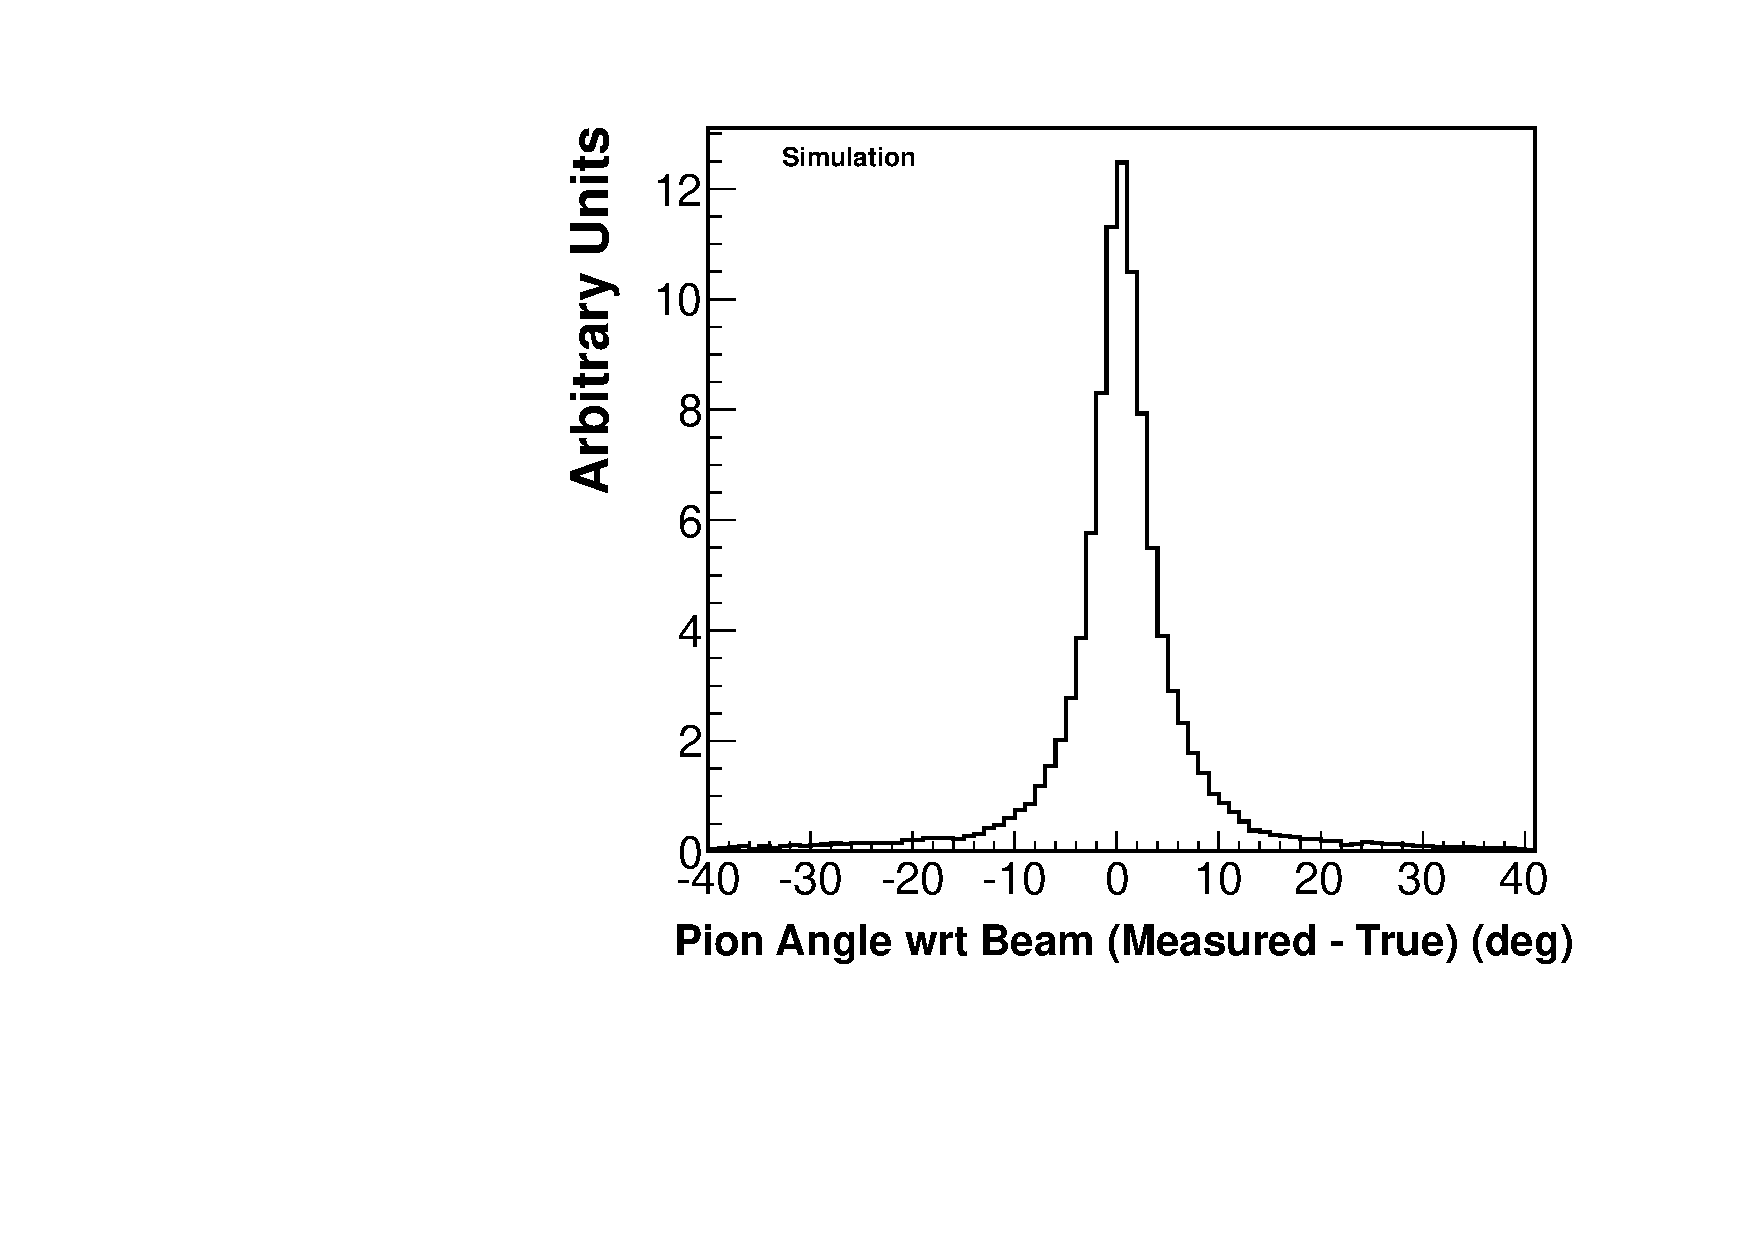
\includegraphics[width=\columnwidth]{figures/resid_pi_theta}
\else
 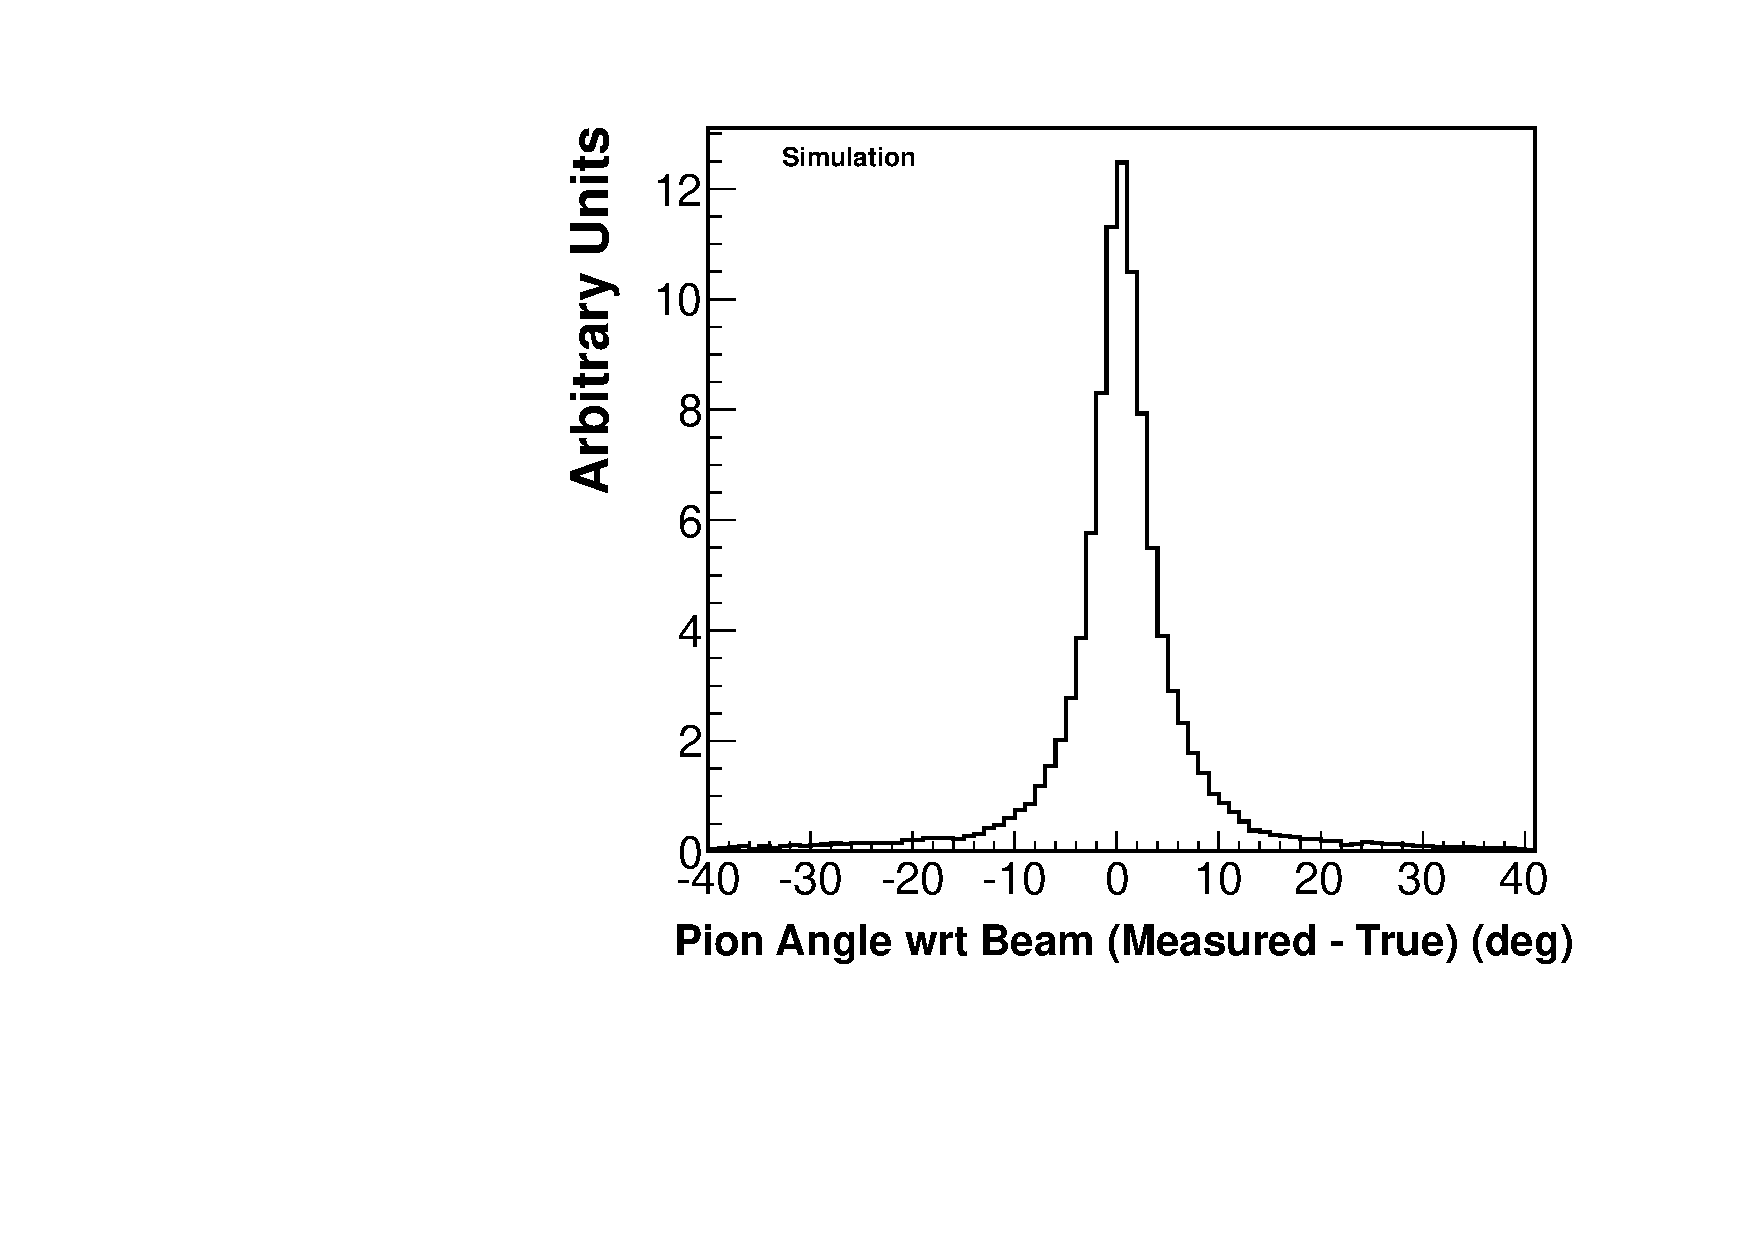
\includegraphics[width=0.99\columnwidth]{figures/resid_pi_theta} % shrink to fit PL 
\fi
    \vspace{-7pt}
\caption{The resolution of the pion angle with respect to the neutrino beam.  Only pions 
from events selected by the \ccpi event selection are included.  The full width at half maximum is 5$^\circ$.}
    \vspace{-10pt}
\label{fig:pi_ang_resid}
\end{figure}

Neutrino event candidates are reconstructed by finding the longest track in the event, then 
searching for additional tracks that share a common vertex with the longest track.  Kinked tracks, which are often the 
result of secondary interactions, are reconstructed by iteratively searching for additional tracks 
starting at the endpoint of the previously found tracks.  Tracks that exit the downstream end of 
the \minerva detector are matched to tracks in MINOS found by the independent MINOS reconstruction; if a match is found, 
it is identified as a muon 
track and the event is retained as a $\nu_\mu$ charged-current interaction candidate. Additional tracks that share a common vertex 
with the muon track are hadron track candidates.  The \minos match requirement is greater than 90\% 
efficient for muons with momenta greater than 1.5~GeV and angles with respect to the beam less than 20$^\circ$. 
The muon energy $E_\mu$ and charge reconstruction use the reconstructed track curvature and range in MINOS.  

\subsection{Charged Pion Identification}
All hadron track candidates that are fully contained within the \minerva detector are classified as pion-like or proton-like by 
a particle identification algorithm that fits the pattern of energy deposition along each track to the Bethe-Bloch 
formula under pion and proton hypotheses.  The fit is allowed to ignore the last cluster on the track or extend up to two planes 
beyond the end of the track without penalty, but is otherwise consistent with the range of the track.  This is done to account 
for mis-reconstruction of the track end position.  Contamination from 
overlapping vertex activity biases pion track fits towards the proton hypothesis; this is avoided by finding the 
portion of the track with an energy profile that is consistent with multiple overlapping particles and not including it in the fit. 

The pion range score $s_{\pi}$ is calculated from the $\chi^{2}$ of the best fit under each hypothesis by the equation

\begin{equation}\label{eq:dEdx_score}
s_{\pi} = 1 - \frac{\chi_{\pi,DOF}^{2}}{\sqrt{\chi_{\pi,DOF}^{4} + \chi_{p,DOF}^{4}}},
\end{equation}
where  $\chi_{\pi,DOF}^{2}$ is the pion best fit $\chi^{2}$ per degree of freedom and $\chi_{p,DOF}^{2}$ is the proton 
best fit $\chi^{2}$ per degree of freedom.  Figure~\ref{fig:pi_score} presents the $s_{\pi}$ distribution of hadronic track 
candidates in events passing the muon and calorimetric \ccpi selections described in Section~\ref{sec:ev_rec}.  Tracks with 
$s_{\pi}>0.6$ are identified as charged pion candidates.  The kinetic energy of the 
best pion fit determines the reconstructed \Tpi, which can be as low as 35~MeV when the best fit does not include the last cluster 
on the track.  The \Tpi resolution is shown in Fig.~\ref{fig:pi_ke_resid}. 

\begin{figure}[tp]
\centering
\ifnum\PRLsupp=0
  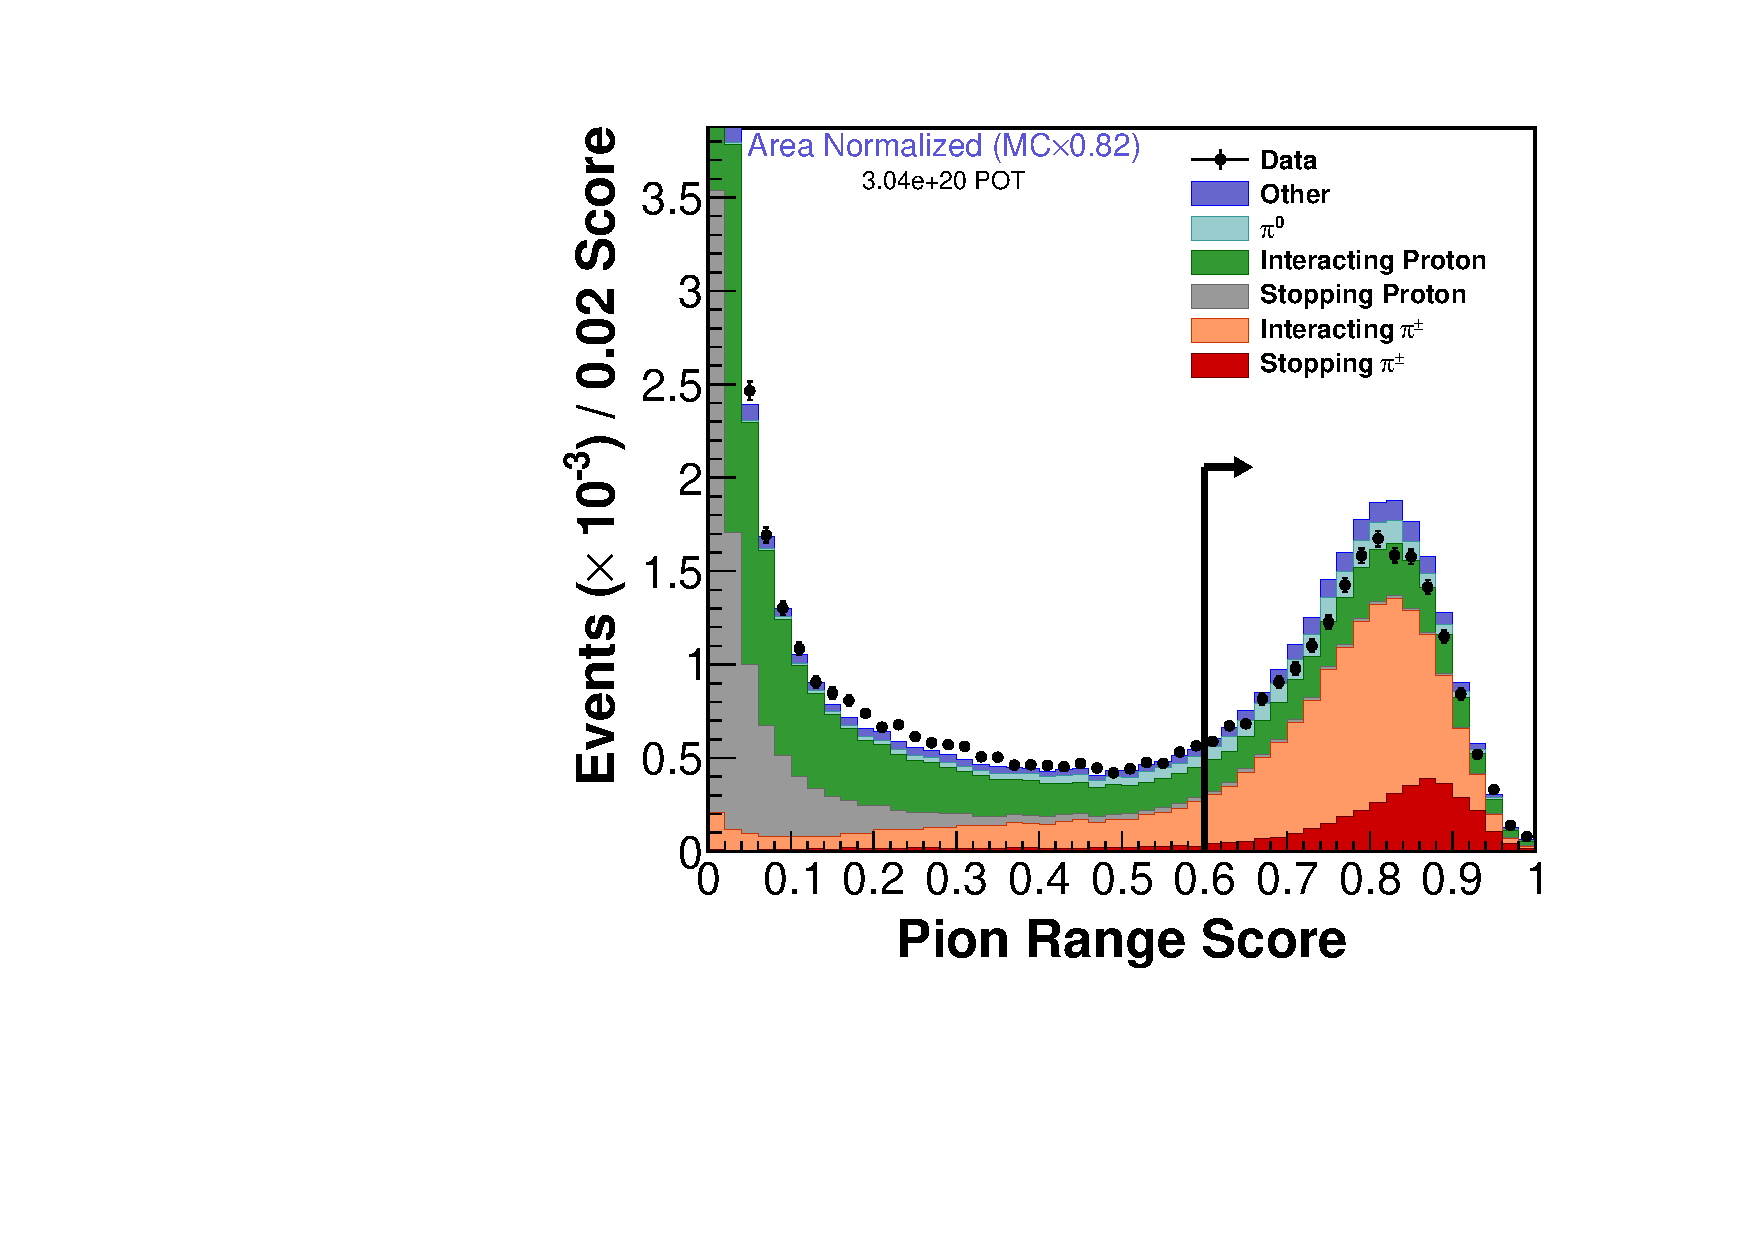
\includegraphics[width=\columnwidth]{figures/pi_dedx_score}
\else
 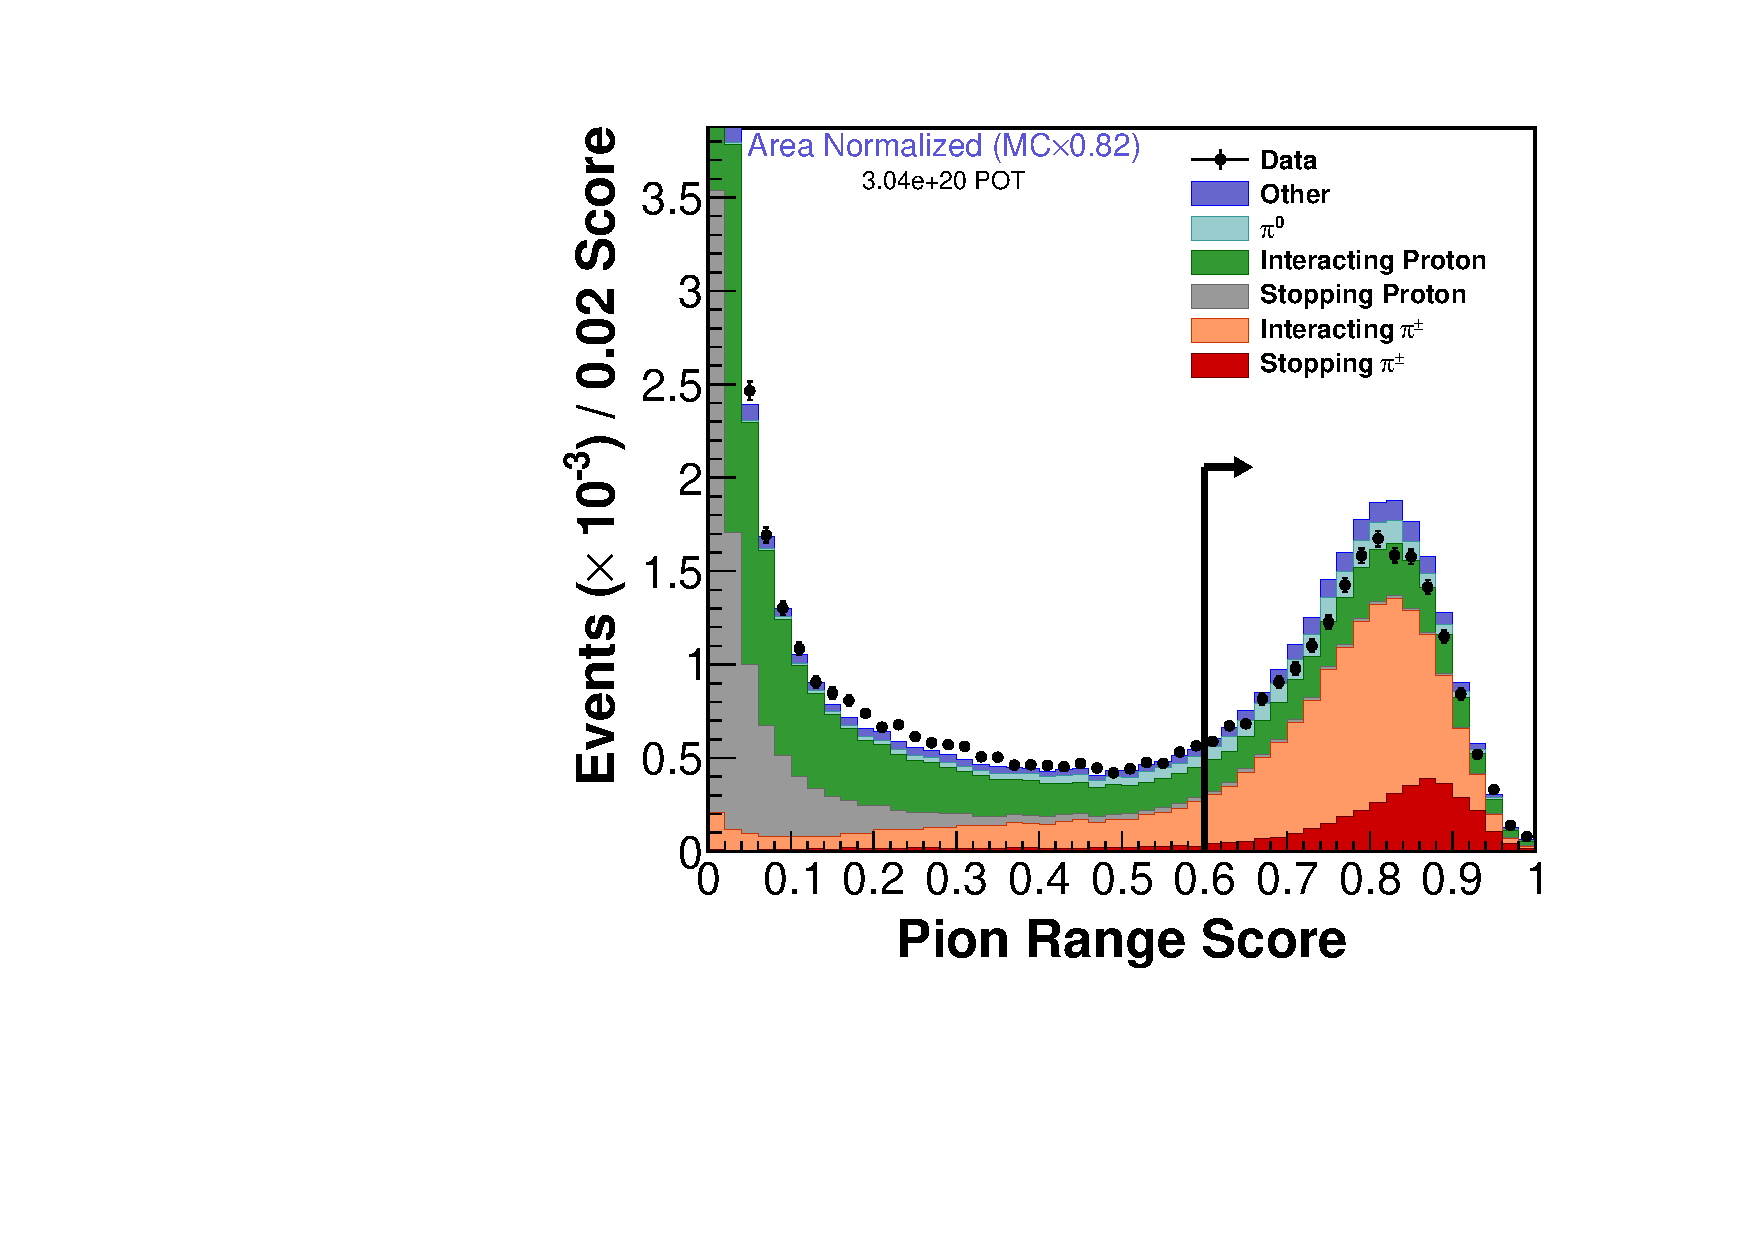
\includegraphics[width=0.99\columnwidth]{figures/pi_dedx_score} % shrink to fit PL 
\fi
    \vspace{-7pt}
\caption{A data-simulation comparison of the pion range score $s_{\pi}$.  All \ccpi event selections are applied except for the Michel electron 
requirement.  The simulation is multiplied by a factor of 0.82 to match the area of the data.  A stopping particle is defined as one 
which is fully contained in the \minerva detector without experiencing a secondary interaction. }
    \vspace{-10pt}
\label{fig:pi_score}
\end{figure}

\begin{figure}[tp]
\centering
\ifnum\PRLsupp=0
  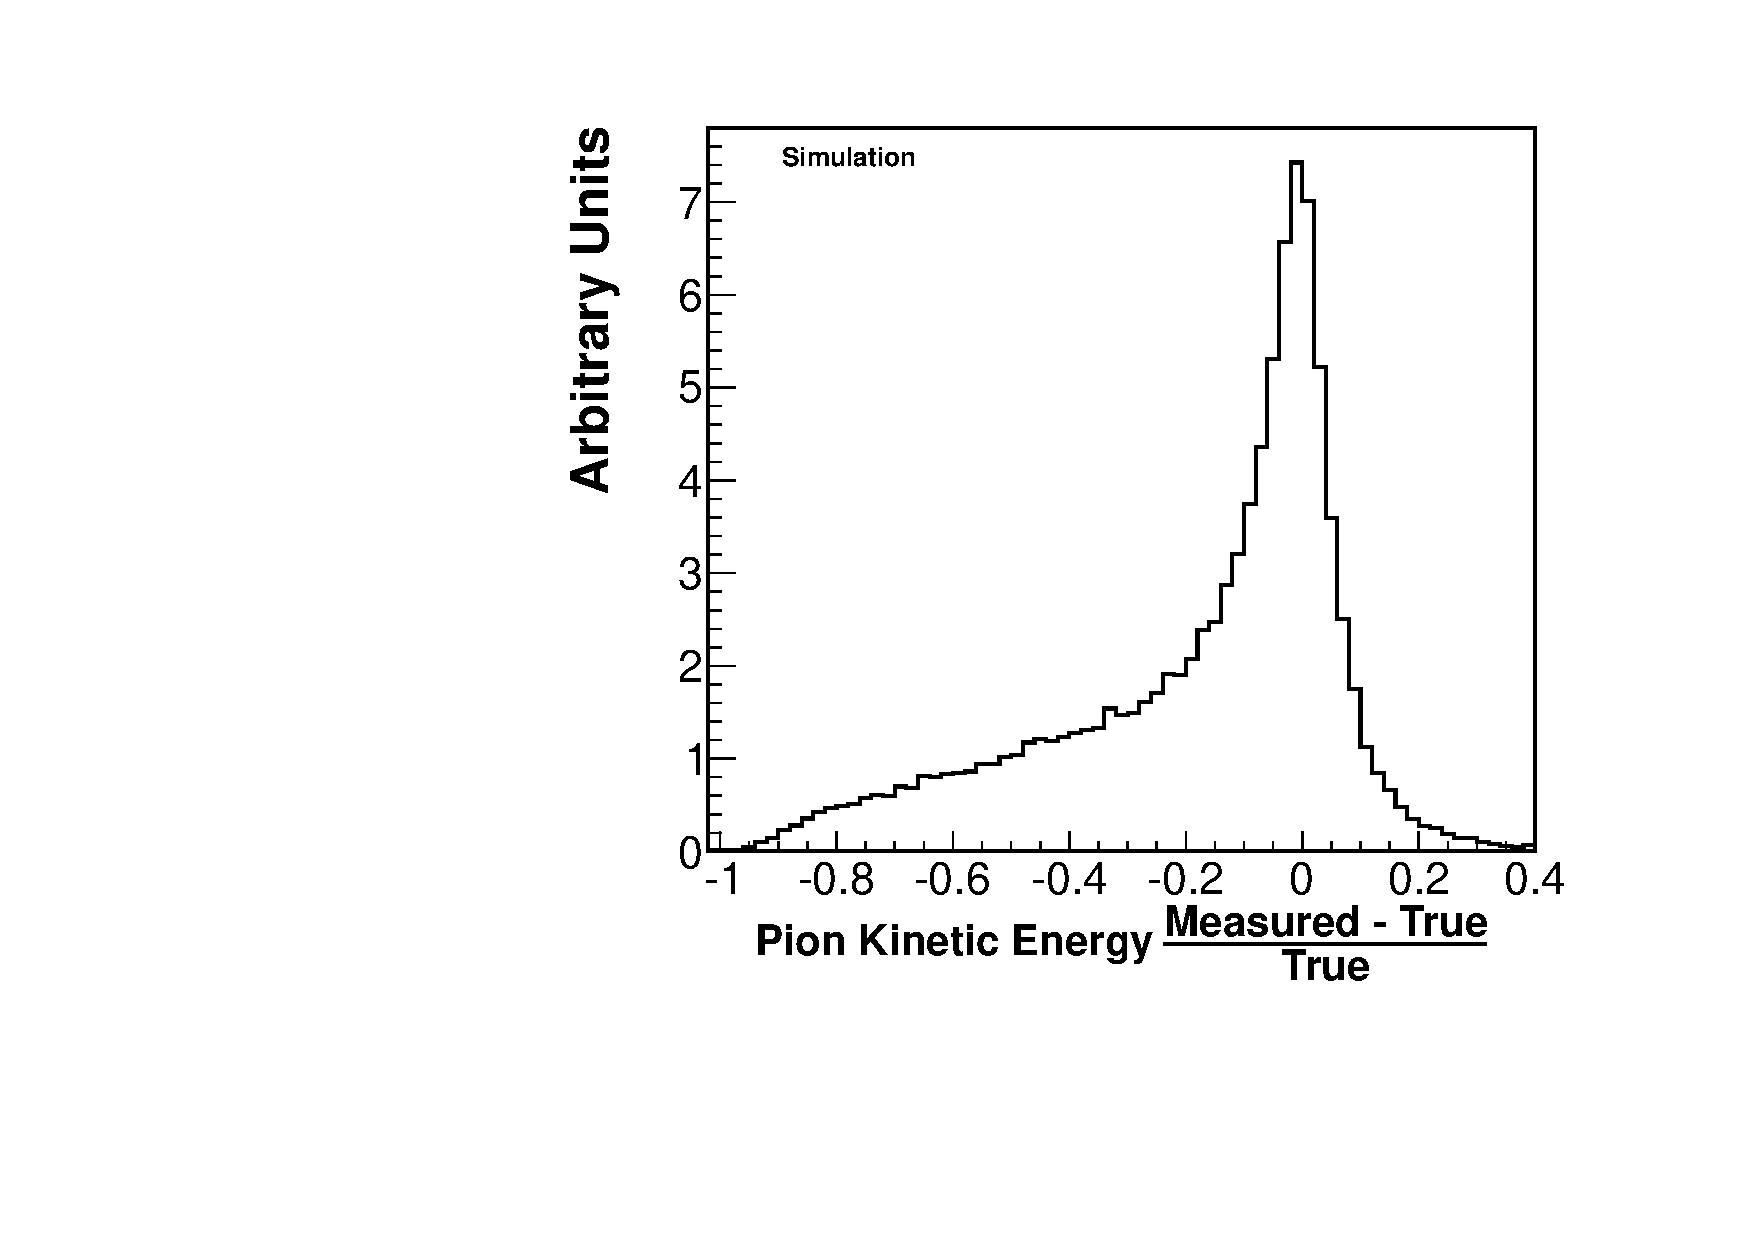
\includegraphics[width=\columnwidth]{figures/resid_pi_ke}
\else
 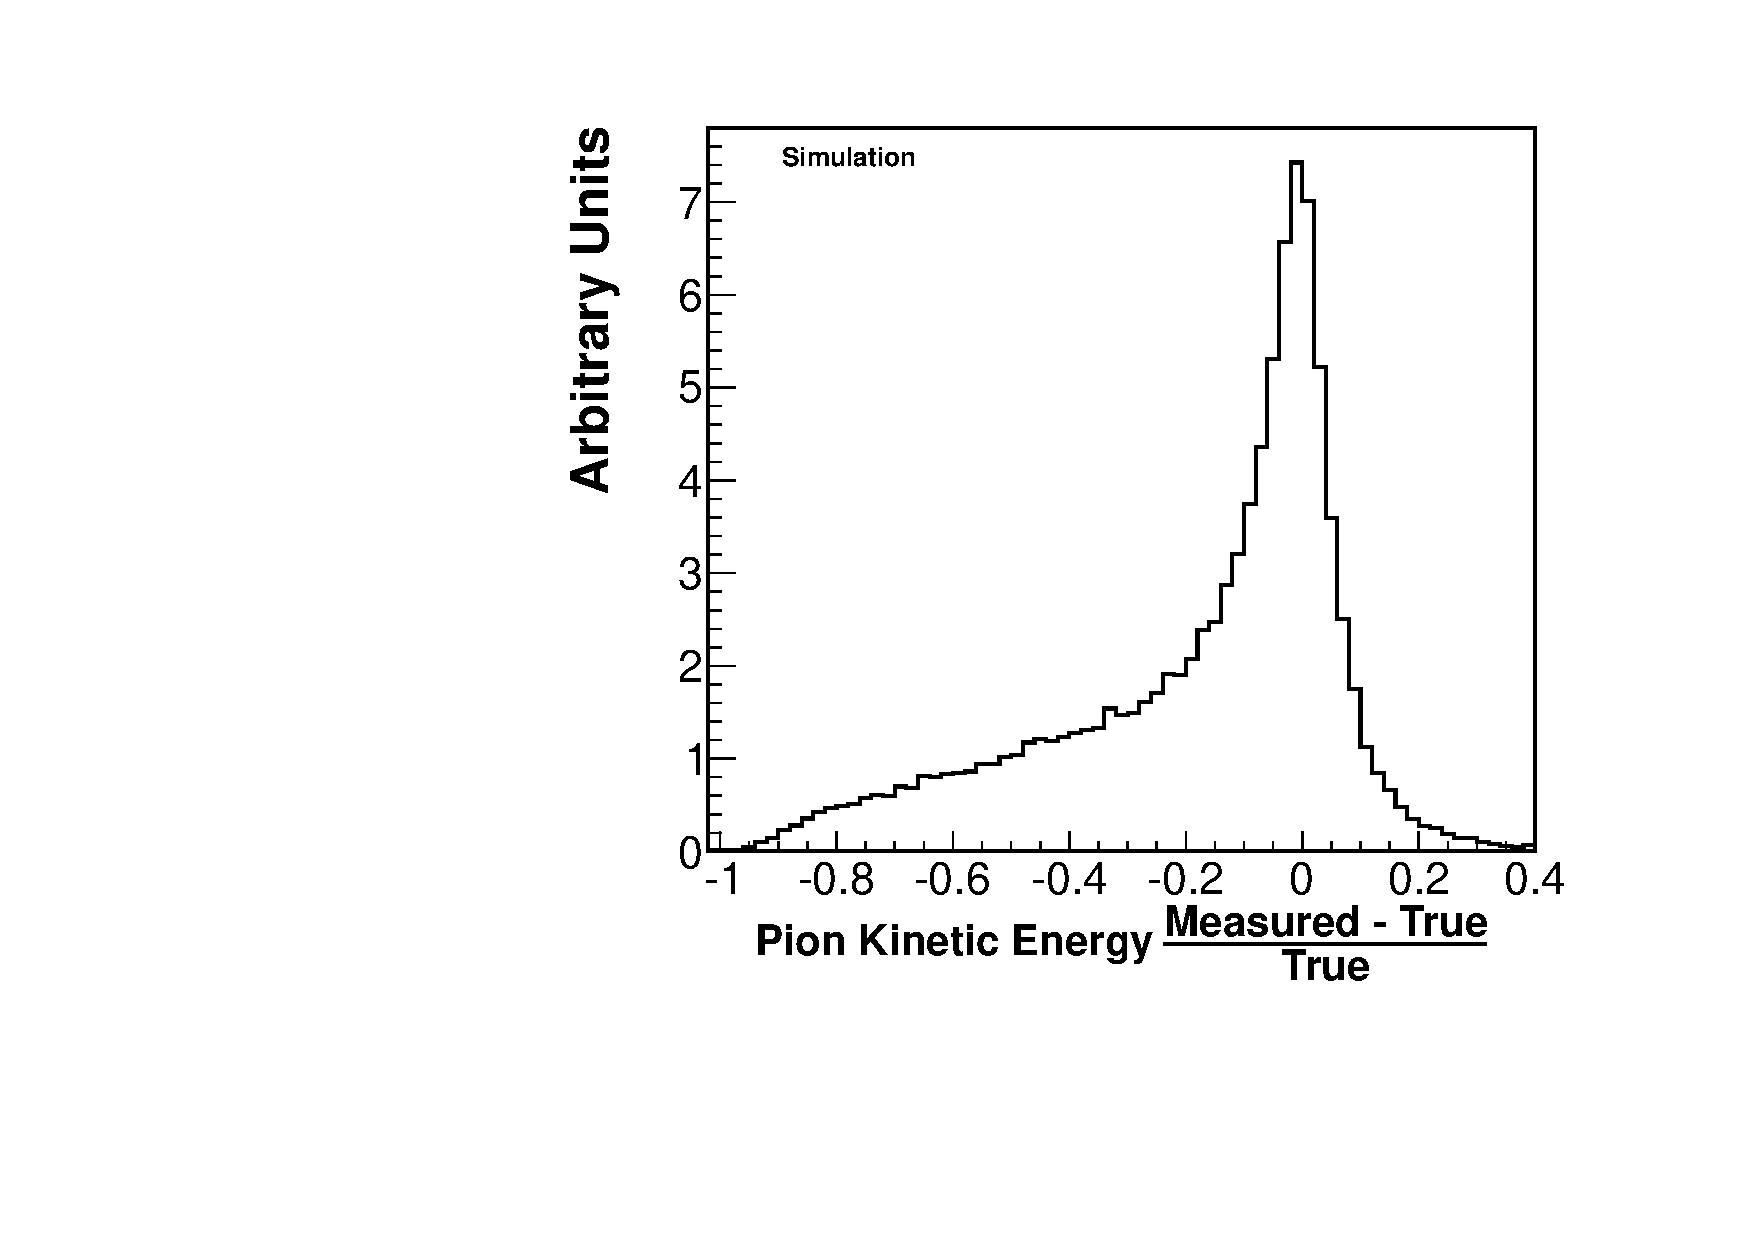
\includegraphics[width=0.99\columnwidth]{figures/resid_pi_ke} % shrink to fit PL 
\fi
    \vspace{-7pt}
\caption{The \Tpi resolution.  Only pions 
from events selected by the \ccpi event selection are included.  The lowside tail consists of inelastic secondary interactions 
with a charged pion in the final state.}
    \vspace{-10pt}
\label{fig:pi_ke_resid}
\end{figure}

Charged pions are also identified by the Michel electron from the $\pi\rightarrow \mu \rightarrow e$ decay chain.  Michel 
candidates are found by searching for delayed energy deposits in each view within a $35 \times 25$~cm$^{2}$ (transverse $\times$ 
longitudinal) box centered on the end position of each hadron track.  The large search box accounts for track mis-reconstruction 
and the potential size of the Michel shower, but will often include energy from unrelated neutrino-induced activity 
that occurs later in the beam spill.  To avoid this, the total visible energy of the Michel candidate must be less than 55~MeV and 
the total number of scintillator strips cannot exceed 35.  These restrictions are motivated by the well-understood kinematics 
of muon decay.  Figure~\ref{fig:michel} shows a comparison of the reconstructed Michel 
visible energy spectrum in data and simulation for pion candidates with $s_{\pi}>0.6$ in \ccpi candidate events.  The means of the data 
and simulation are consistent within the 3\% uncertainty on the detector energy response to electromagnetic 
particles.  Michel candidates are associated with an at-rest $\pi^{+}$ with an efficiency of 80\%, as validated
in data with stopped muons from upstream neutrino interactions.

\begin{figure}[tp]
\centering
\ifnum\PRLsupp=0
  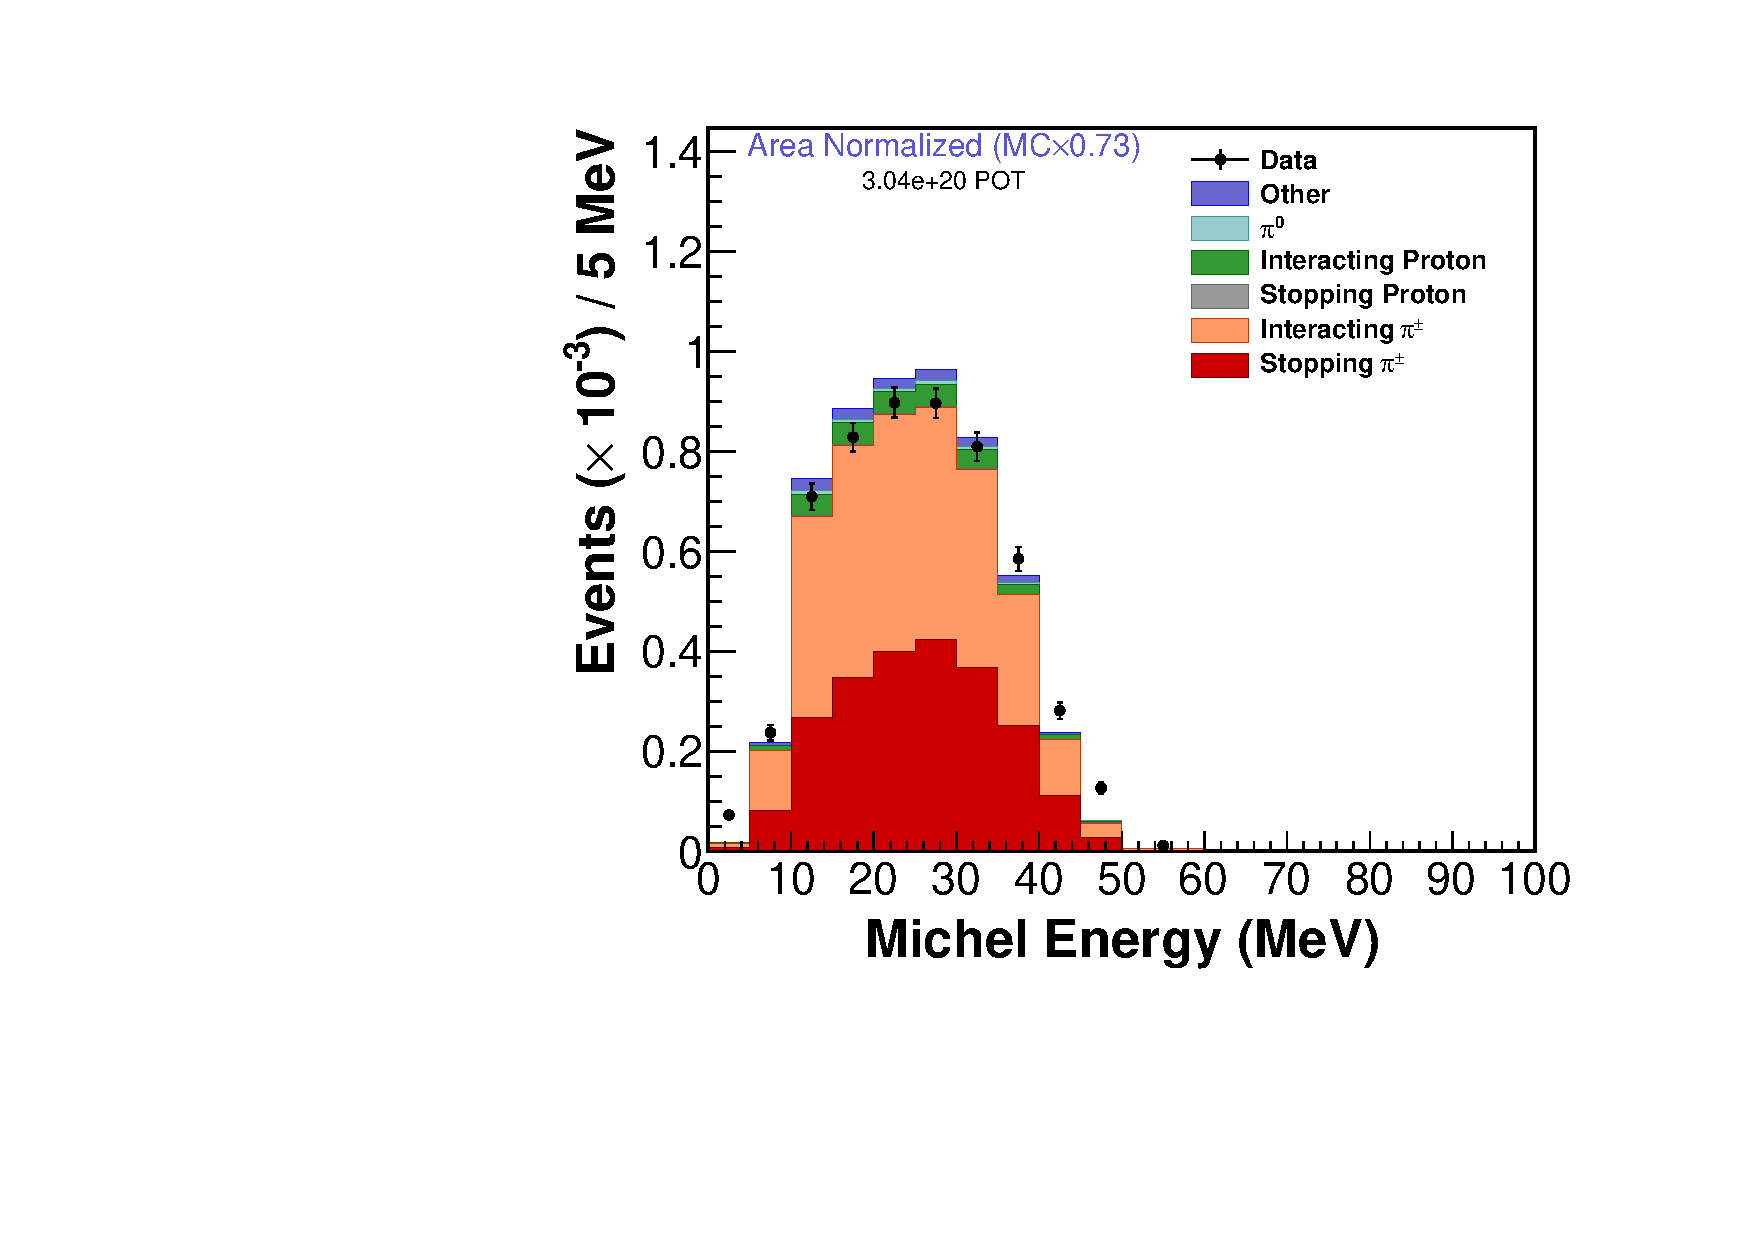
\includegraphics[width=\columnwidth]{figures/michel_e_an}
\else
 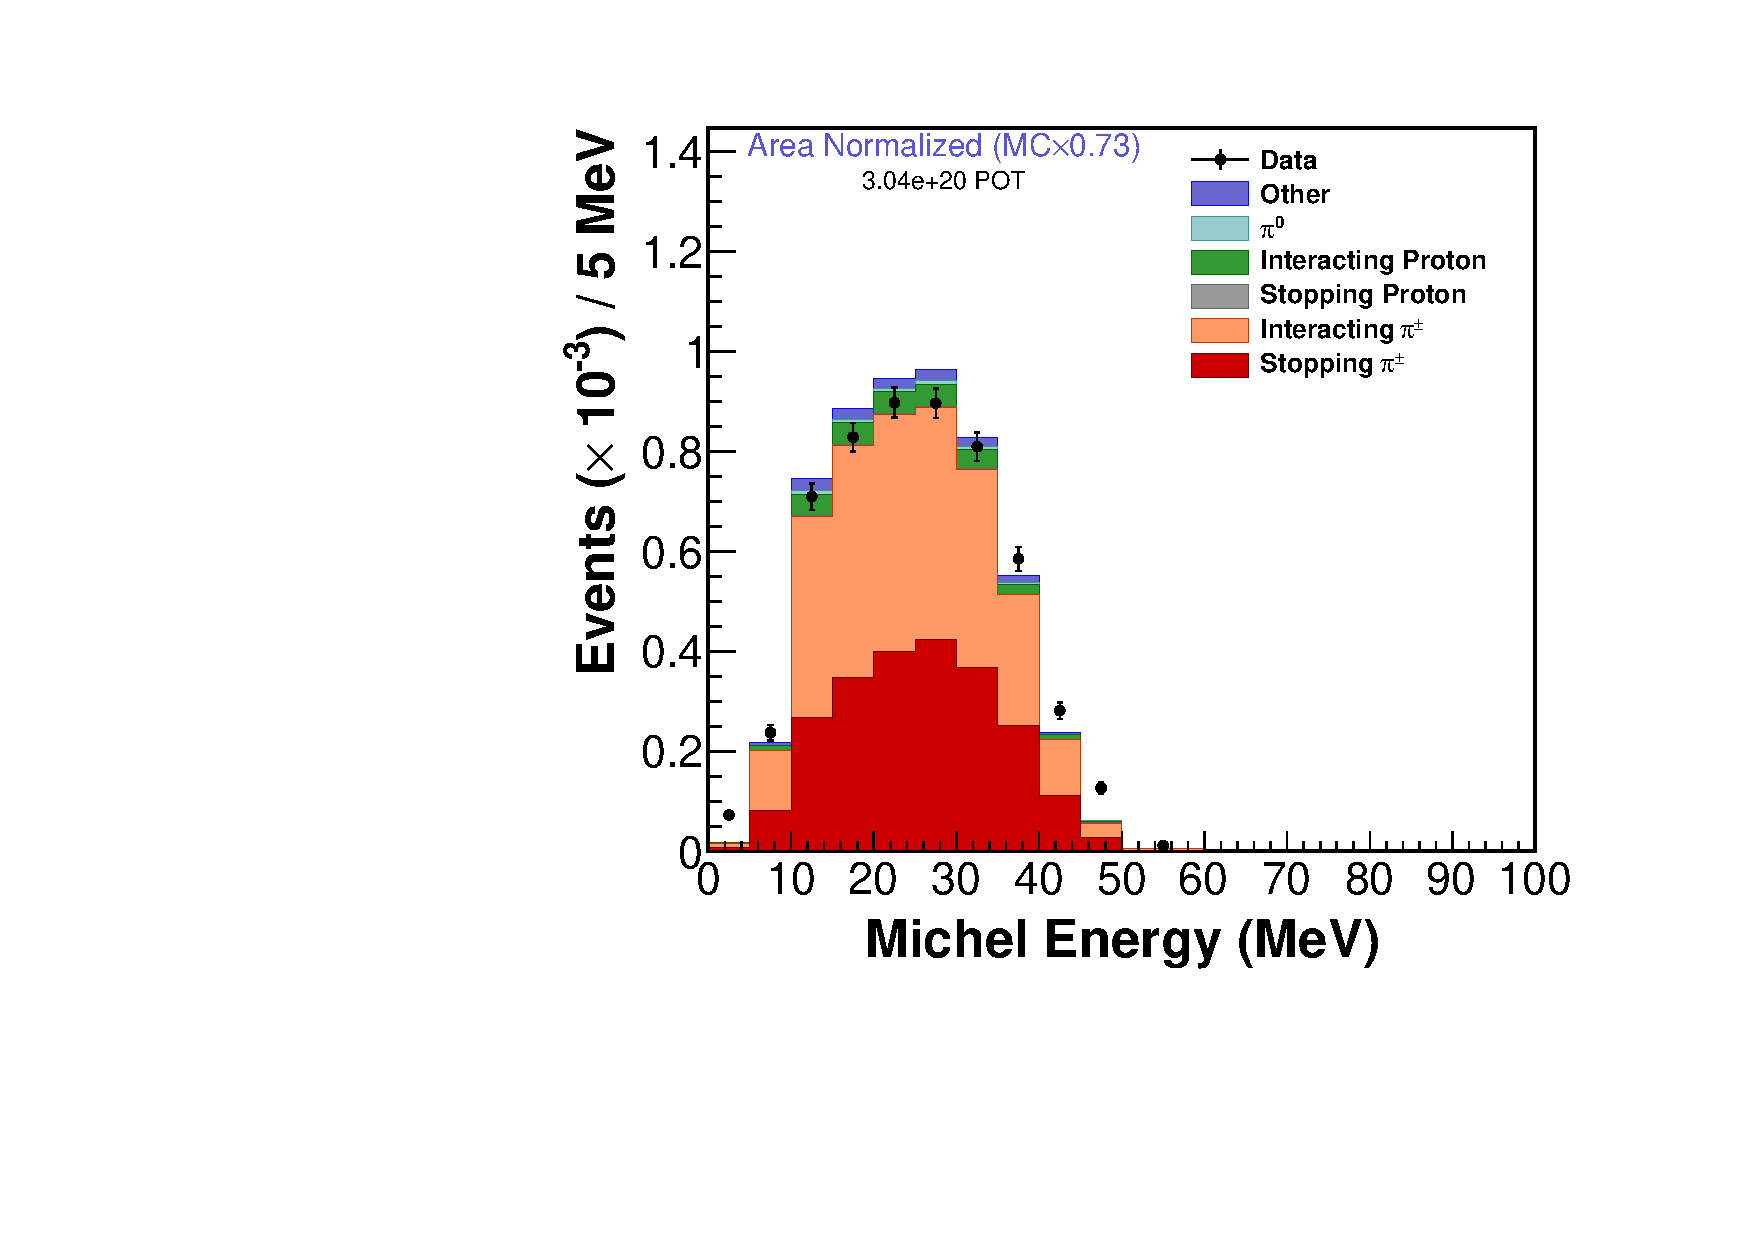
\includegraphics[width=0.99\columnwidth]{figures/michel_e_an} % shrink to fit PL 
\fi
    \vspace{-7pt}
\caption{The visible energy distribution of Michel candidates selected by the \ccpi analysis.  The simulation is scaled by a factor of 0.73 to match 
the area of the data.}
    \vspace{-10pt}
\label{fig:michel}
\end{figure}
 
\subsection{Neutrino Energy Reconstruction} 
The neutrino energy in \ccpi events can be reconstructed kinematically using the reconstructed four-momentum of the muon and pion, 
but this requires the assumptions that there is only one nucleon in the final state and that the pion did not experience FSI. Instead, 
this analysis employs a calorimetric energy reconstruction that utilizes the final-state recoil energy $E_\mathrm{recoil}$ 

\begin{equation}\label{eq:e_recoil_def}
E_\mathrm{recoil} \equiv E_\nu - E_\mu,
\end{equation}
which is reconstructed as the calorimetrically-weighted sum of the visible energy not associated with the muon track, i.e.

\begin{equation}\label{eq:e_recoil_rec}
E_\mathrm{recoil} = \beta\left(\alpha\sum\limits_{i} C_{i}E_{i}\right),
\end{equation}
where $E_{i}$ is the non-muon reconstructed energy in subdetector $i$ (the tracking detector, downstream electromagnetic calorimeter, downstream hadronic
calorimeter, and the outer calorimeter), $C_{i}$ is a calorimetric constant determined by the fraction of 
passive material in subdetector $i$, and $\alpha$ and $\beta(E)$ are model-dependent parameters, tuned to the true $E_\mathrm{recoil}$ using a 
simulated charged-current interaction sample, that account for undetected energy from neutral and exiting particles.  

Neutrino energy and other kinematic quantities are calculated from $E_\mathrm{recoil}$ and the reconstructed muon four-momentum using 
the following equations:
\begin{eqnarray}
E_\nu &=& E_\mu + E_\mathrm{recoil},\\
Q^2 &=& 2E_\nu(E_\mu-|\vec{p}_\mu|\cos(\theta_\mu))-m_\mu^2,\\
W_{exp}^2 &=& M_p^2 - Q^2 + 2M_pE_\mathrm{recoil}. \label{eq:Wexp_rec}
\end{eqnarray}
Here, $M_p (m_\mu$) is the proton (muon) mass, $p_\mu$ and $\theta_\mu$ are
the reconstructed momentum and angle of the muon with respect to the beam, and the $W_{exp}$ is $W$ calculated with the assumption of a single free 
target nucleon at rest.  Of the three quantities above, $W_{exp}$ is most important for this analysis.  The $W_{exp}$ resolution 
in selected \ccpi events are shown in Fig.~\ref{fig:Wexp_resid}.
The resolution on $W_{exp}$ is about 8.5\% with a bias of $-5\%$.  The bias is the result of using an inclusive sample of 
charged-current events, which have a higher average 
multiplicity than \ccpi events restricted to $W<1.8$~GeV, to tune $E_\mathrm{recoil}$.

\begin{figure}[tp]
\centering
\ifnum\PRLsupp=0
  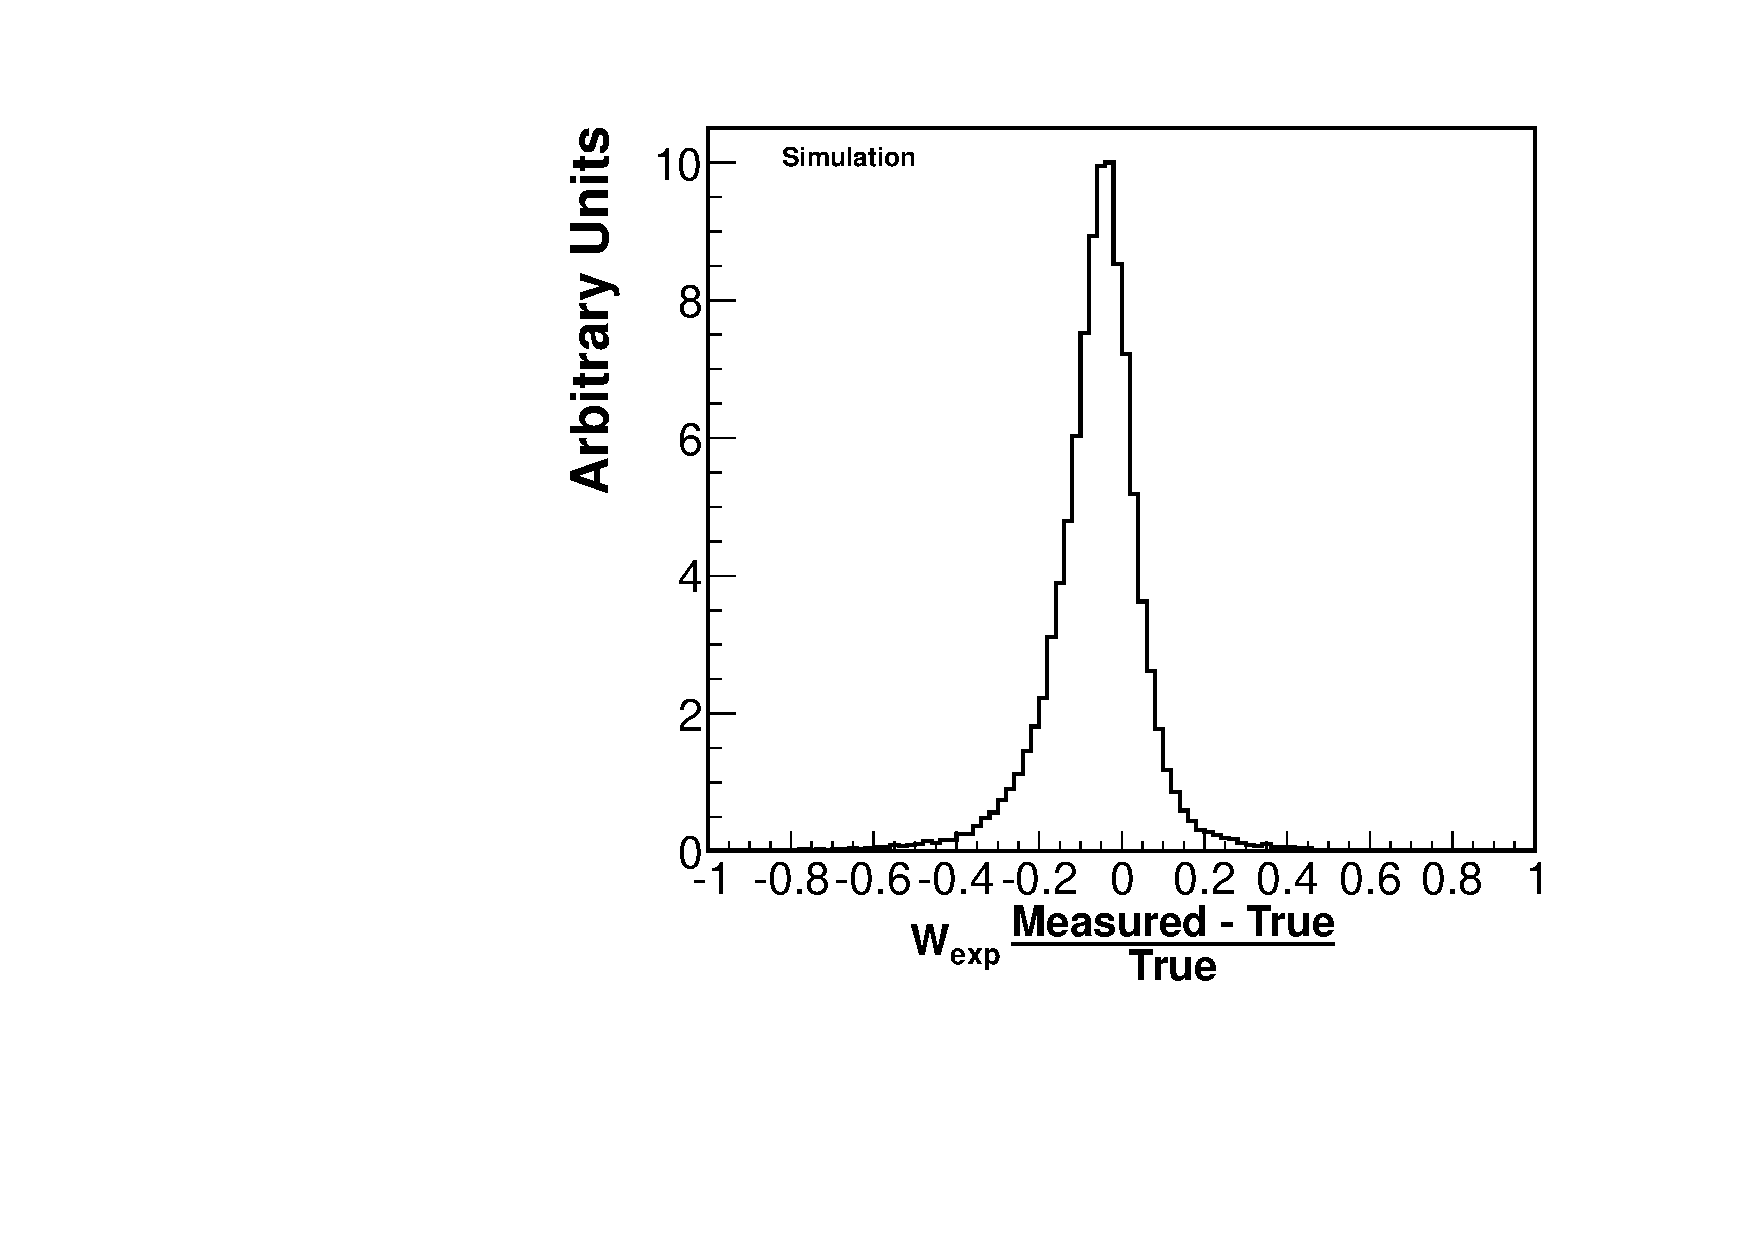
\includegraphics[width=\columnwidth]{figures/resid_W}
\else
 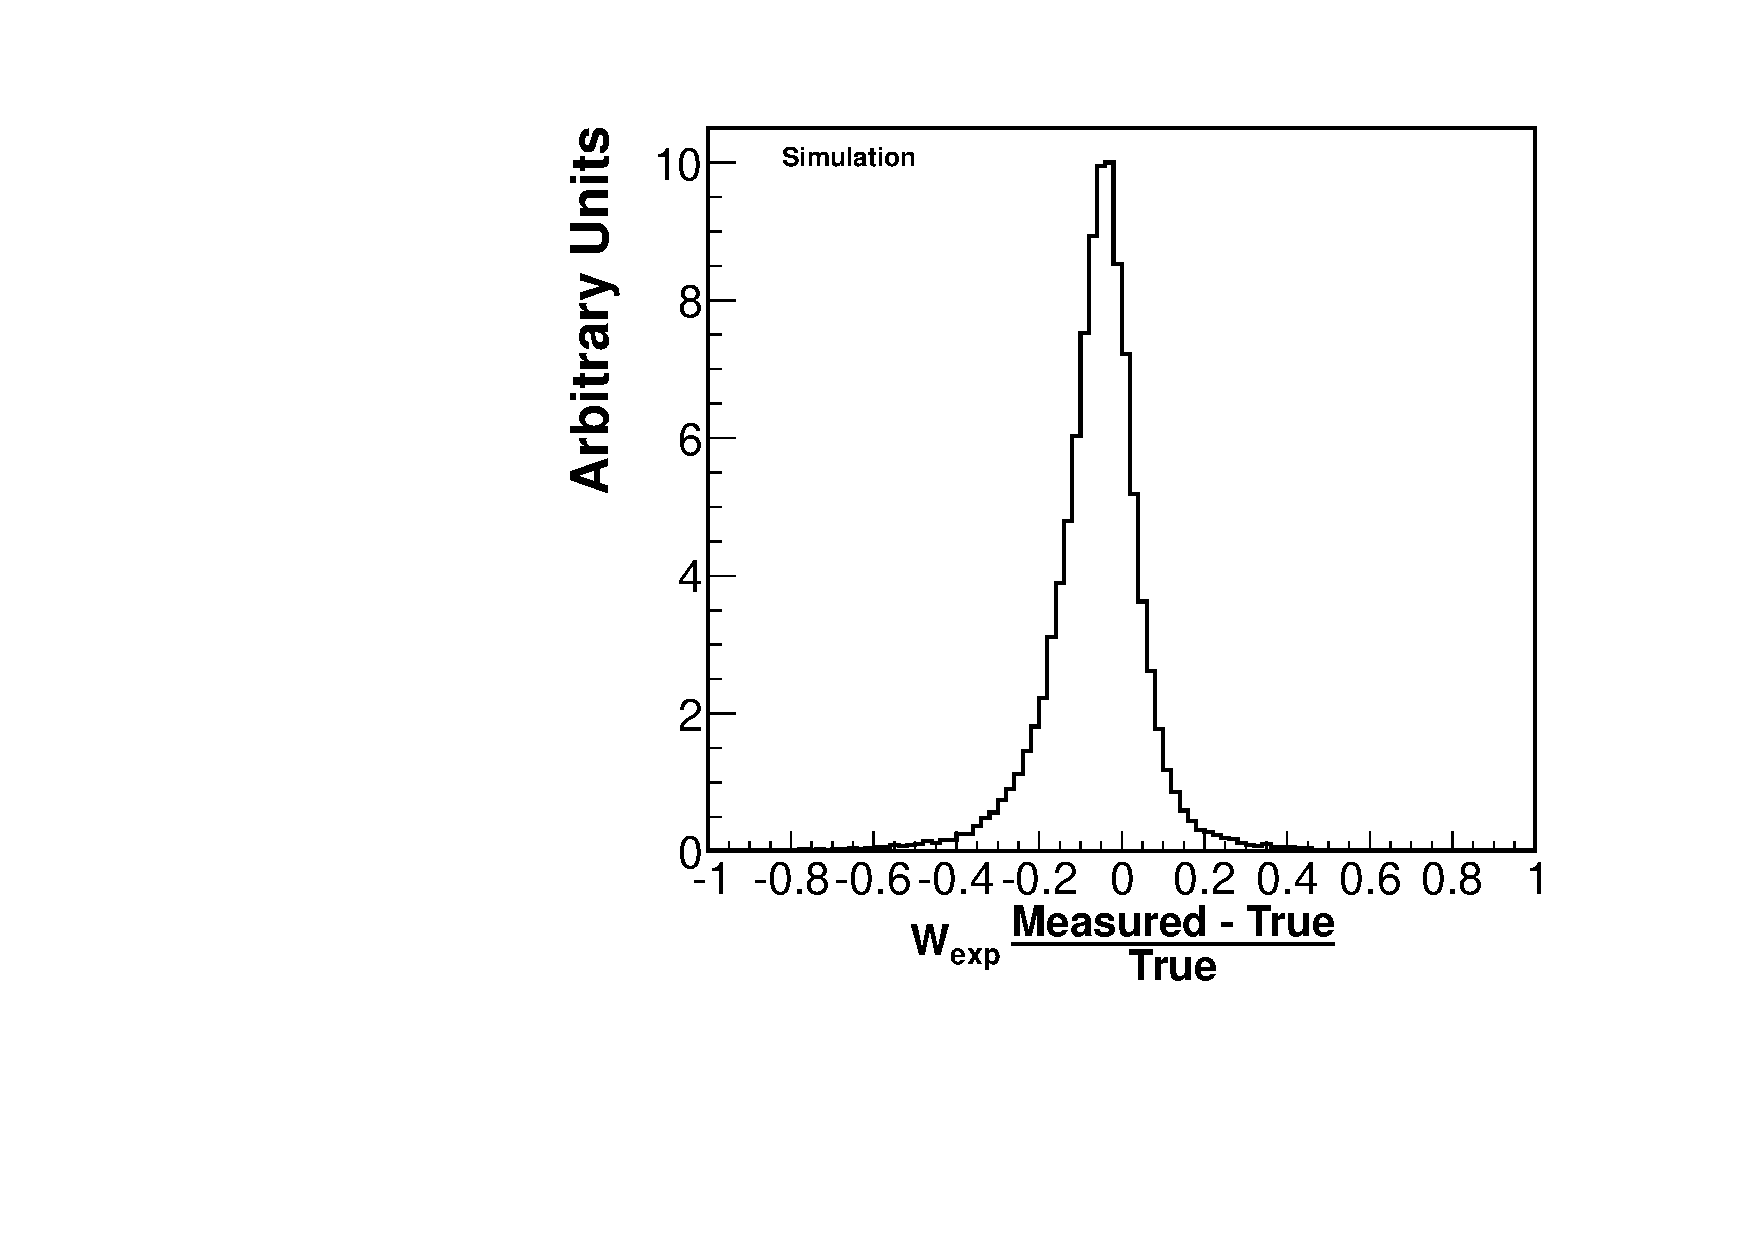
\includegraphics[width=0.99\columnwidth]{figures/resid_W} % shrink to fit PL 
\fi
    \vspace{-7pt}
\caption{The $W_{exp}$ resolution, in which true refers to $W_{exp}$ calculated by using 
true quantities in \eqref{eq:Wexp_rec}.  Only 
events selected by the \ccpi event selection are included.  The full width at half maximum is 17\%}
    \vspace{-10pt}
\label{fig:Wexp_resid}
\end{figure}

\section{Event Selection} 
\label{sec:ev_rec}
Reconstructed \cconepi (\ccpi) events are required to contain one negatively-charged muon track and exactly one (at least one) charged-pion track 
joined at a common vertex.  The event vertex is 
restricted to occur within the central 110 planes of the scintillator tracking region and 
at least \unit[22]{cm} from any edge of the planes. These requirements define a 
fiducial region with a mass of \unit[5.57]{metric tons}, containing $(3.54 \pm 0.05) \times 10^{30}$ nucleons.

Charged pion tracks are identified by a containment requirement and two particle identification selections.  Each pion track 
is required to begin at the event vertex and stop in either the tracking or electromagnetic calorimeter regions 
of \minerva, which restricts the maximum pion kinetic energy to 350~MeV.  The particle identification selections require that there exist at 
least one track with $s_\pi>0.6$ and  
an associated Michel electron candidate.  The Michel selection disfavors 
both negatively-charged pions, which tend to be captured on a nucleus before decaying, and pions that experience secondary interactions in the detector.  The
\cconepi (\ccpi) analysis requires exactly (at least) one reconstructed charged pion track.

The reconstructed $E_\nu$ is required to be between 1.5 and 10 GeV in both analyses.  The lower bound of this selection is 
made to match the \minos muon acceptance threshold.  The upper bound reduces 
flux uncertainties, which are largest above 10~GeV.  The \cconepi analysis 
selects events with $W_{exp}<1.4$ GeV, while the \ccpi analysis selects $W_{exp}<1.8$ GeV.

After all selections, 3474 (5410) events remain in the \cconepi (\ccpi) analysis.  Figure~\ref{fig:reco_dist} shows the selected \Tpi and 
\thetapi for both analyses.  There is a large normalization difference between simulation and data that is approximately the size 
of the total uncertainty in the prediction. This uncertainty is dominated by the uncertainty on the normalization of the resonance production cross section in 
neutrino-nucleon scattering, which GENIE determines by combining the ANL and BNL pion production data discussed in Section~\ref{sec:intro}.  
The cross section extraction procedure (see Section~\ref{sec:xs}) is designed to minimize the influence of this model uncertainty on the measured cross section distributions.

\begin{figure*}[ht]
  \centering
  \subfloat[] {
    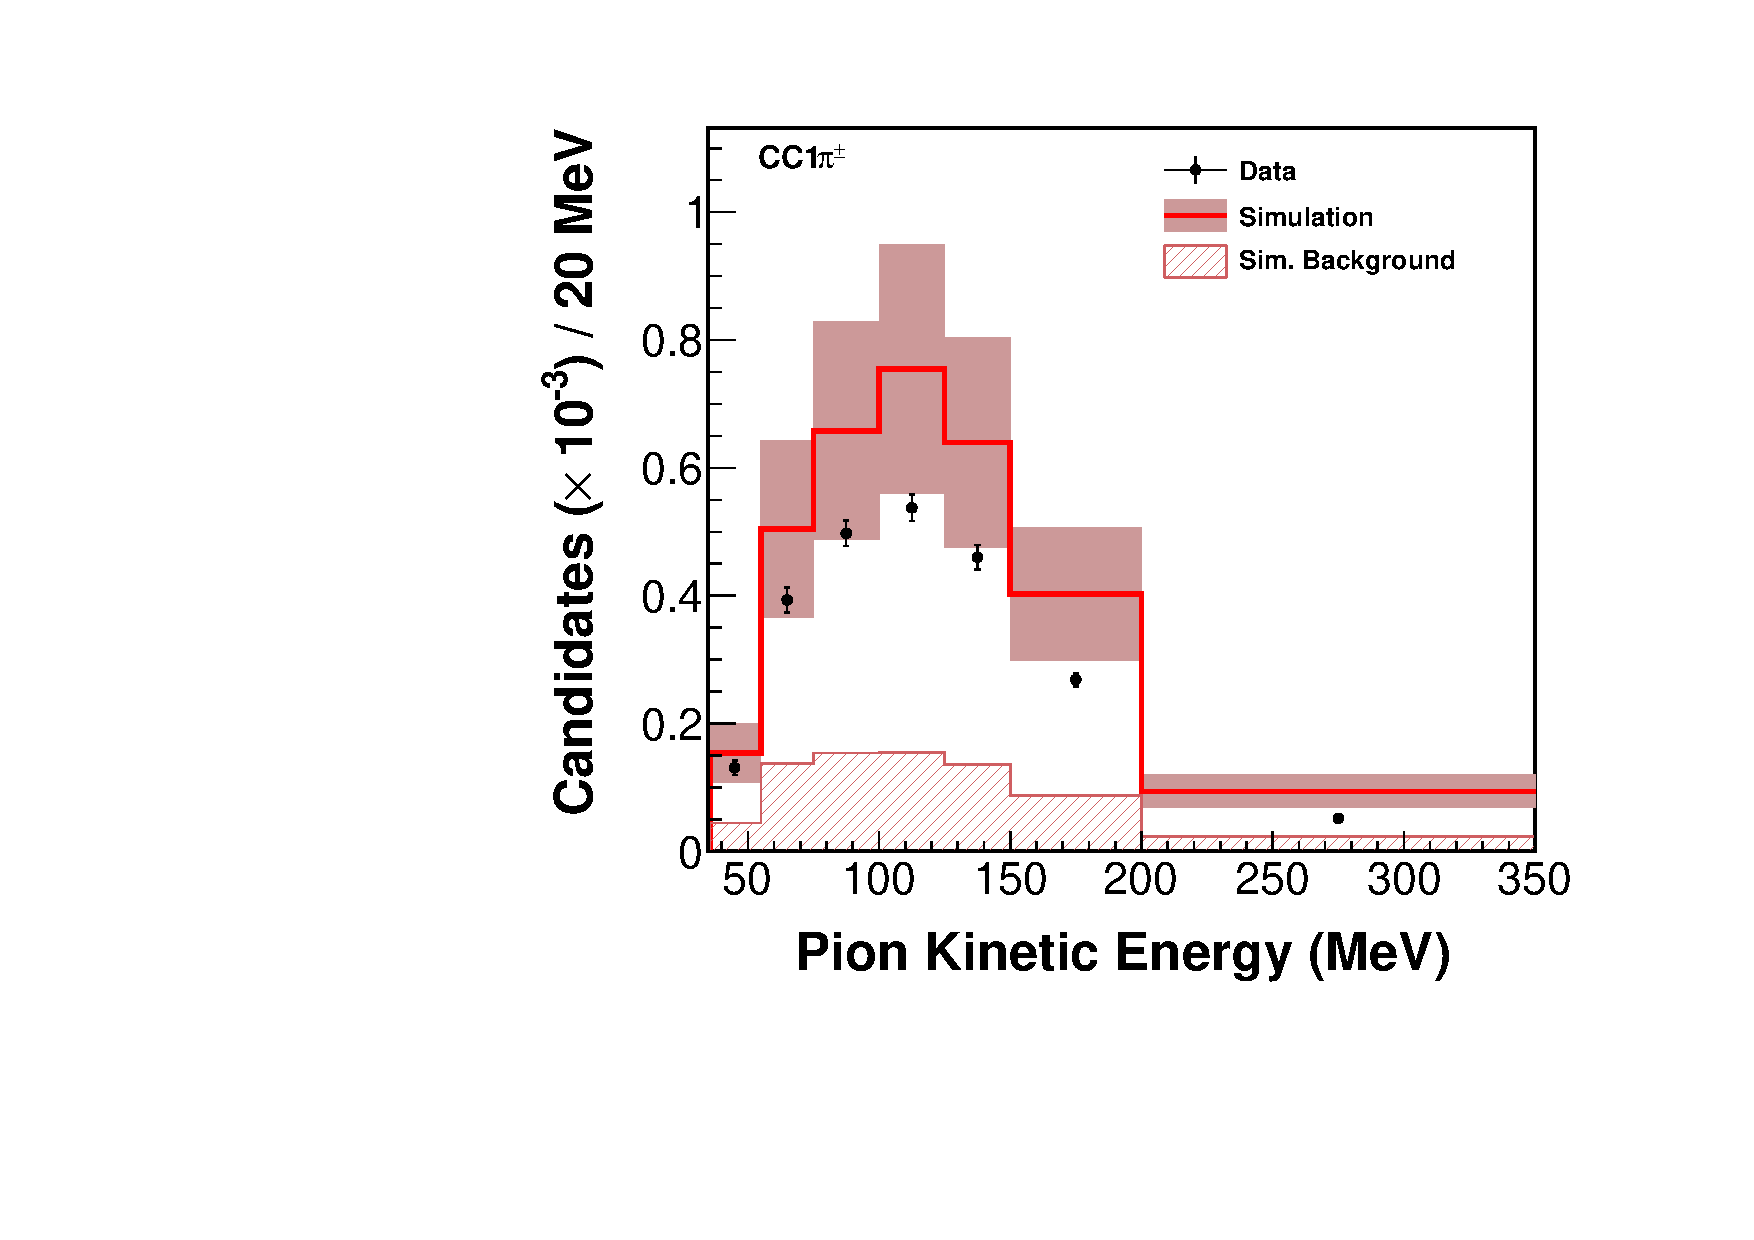
\includegraphics[width=\columnwidth]{figures/comp_pi_ke_pn_1pi}
  }
  \subfloat[] {
    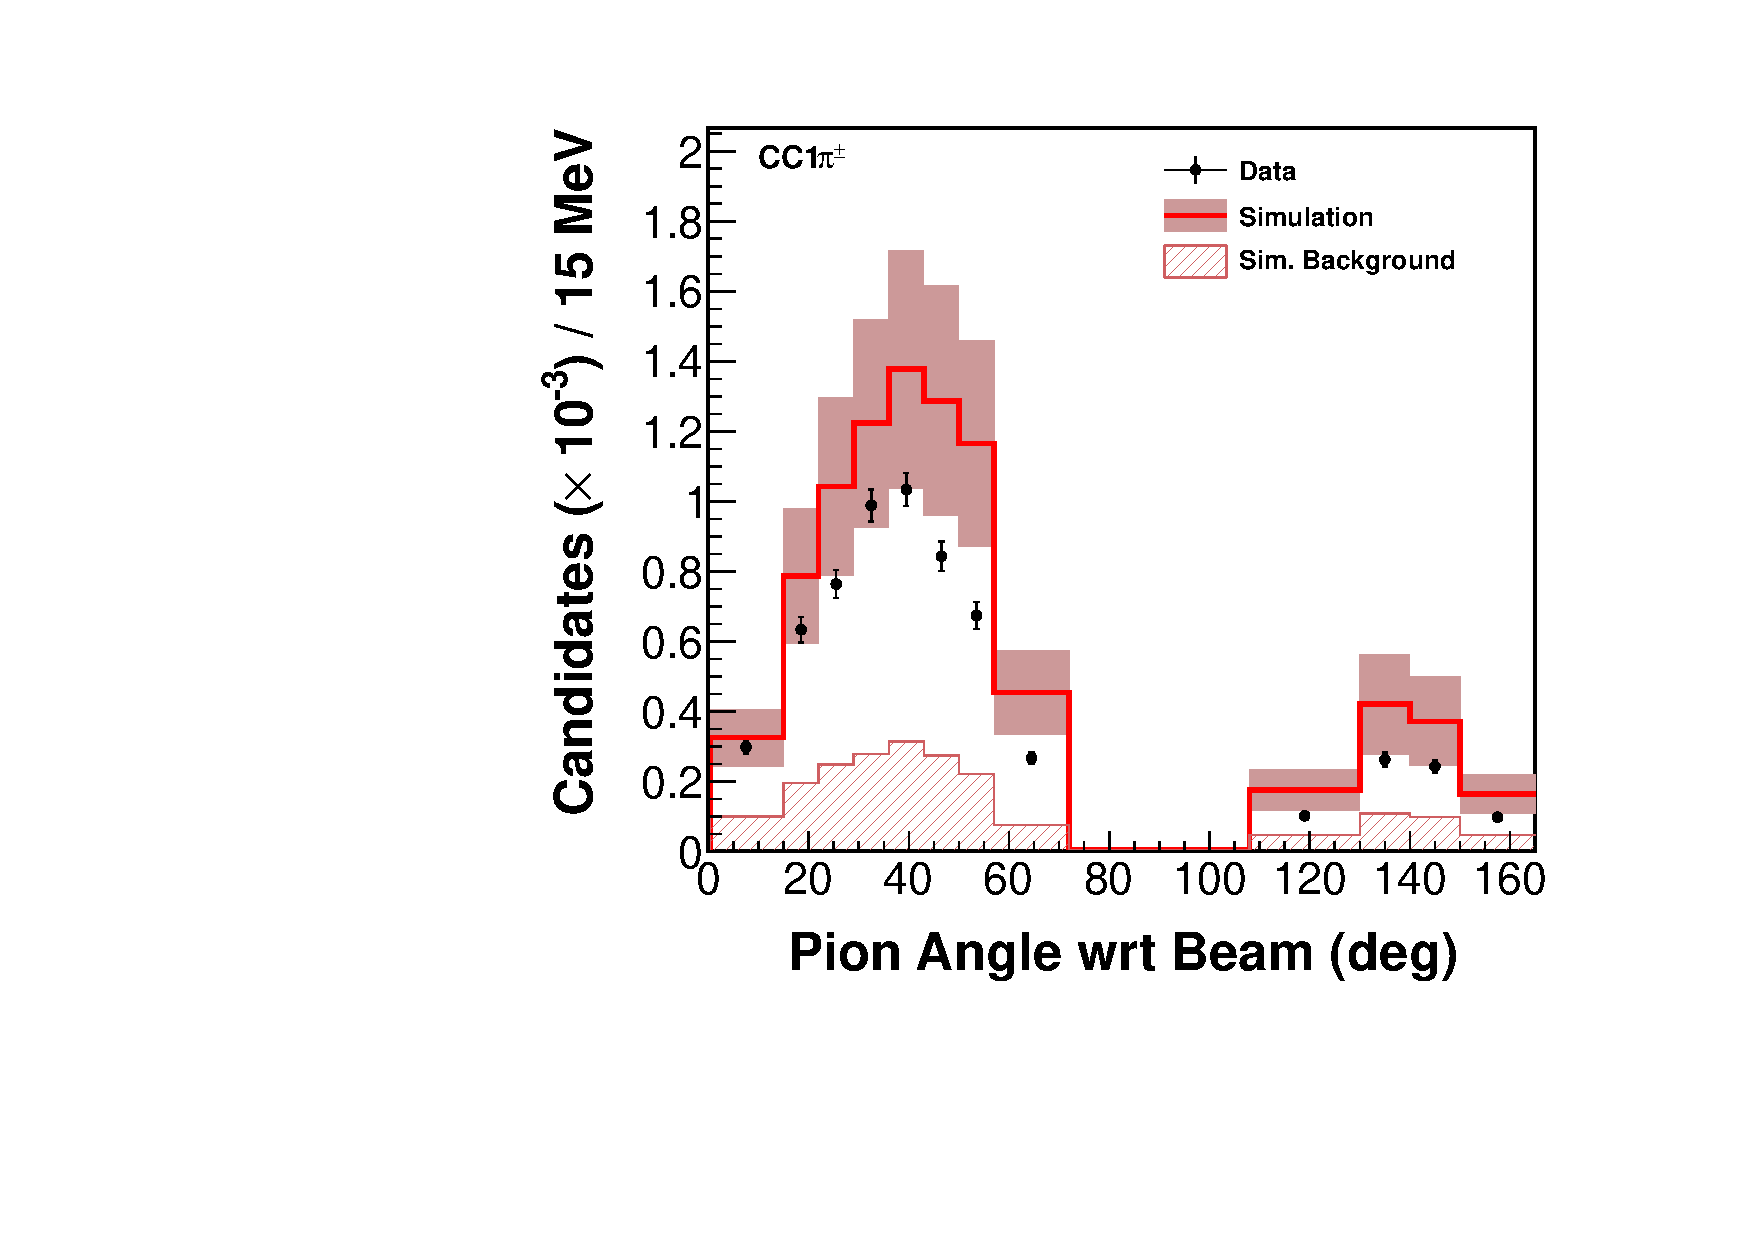
\includegraphics[width=\columnwidth]{figures/comp_pi_theta_pn_1pi}
  }
  \qquad
  \subfloat[] {
    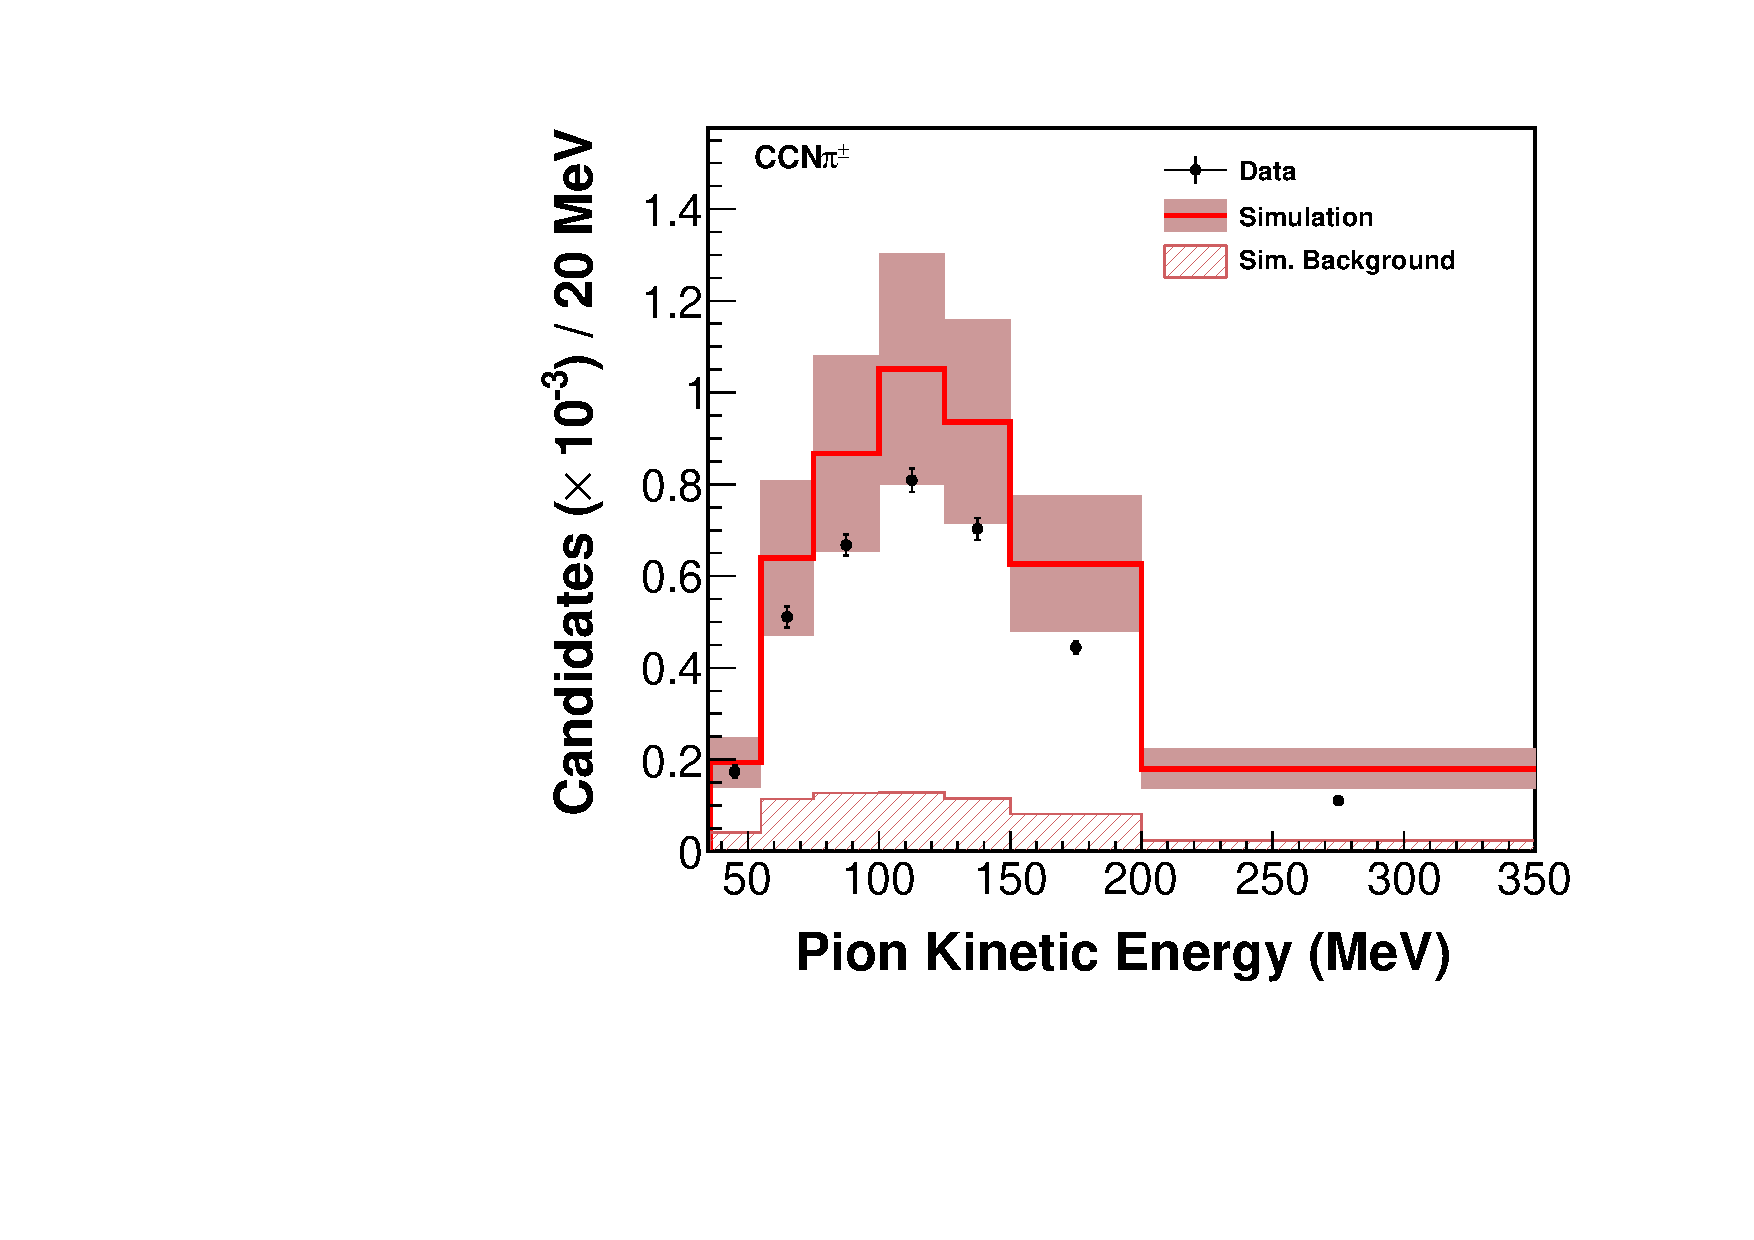
\includegraphics[width=\columnwidth]{figures/comp_pi_ke_pn_Npi}
  }
  \subfloat[] {
    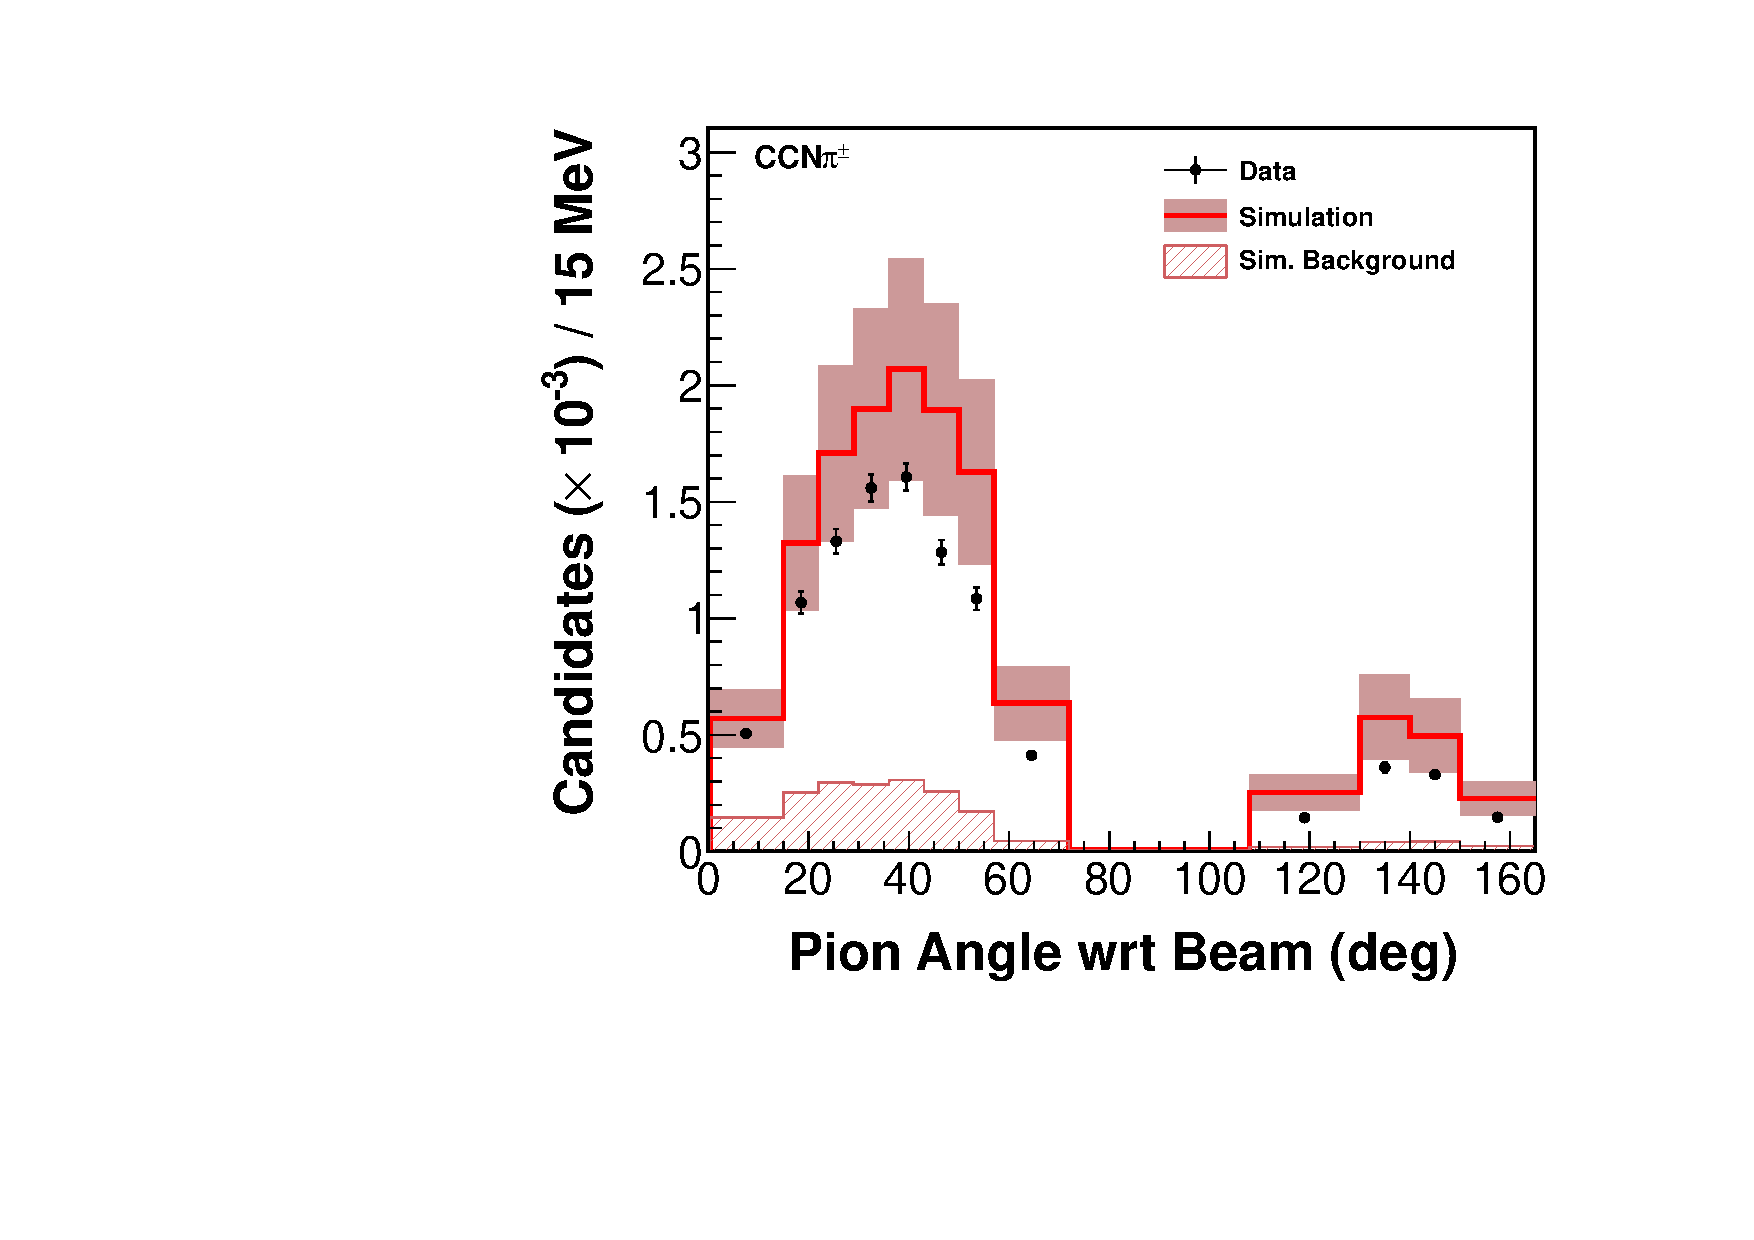
\includegraphics[width=\columnwidth]{figures/comp_pi_theta_pn_Npi}
  }
  \caption{Data-simulation comparisons of the \cconepi (top) and \ccpi (bottom) reconstructed pion kinetic energy and angle distributions after all event selections are applied.}
  \label{fig:reco_dist}
\end{figure*} 

The selected pions are predicted to be 99.6\% 
(98.6\%) $\pi^+$ in the \cconepi (\ccpi) analysis because $\pi^-$ can only arise from FSI 
at low $W$ and are unlikely to survive the Michel electron requirement. The selection efficiency of 
charged pions between 35~MeV and 350~MeV in signal events is determined by simulation to be 4\% (3\%) in the \cconepi (\ccpi) analysis.  
The largest reductions in the selection efficiency are caused by the \minos-matched muon requirement, the pion track reconstruction 
inefficiency, and the Michel electron selection; the latter two are particularly affected by secondary pion scattering and absorption in the 
detector.  The signal purity of the \cconepi (\ccpi) event sample is 77\% (86\%).  Table~\ref{tab:bkgs} summarizes the background components 
in both analyses.  

\begingroup
\squeezetable
\begin{table}
\begin{tabular}{l|c|c}
  \hline\hline
  Background & \cconepi Sample (\%) & \ccpi Sample (\%) \\
  \hline
  $W > 1.4$ GeV ($1.8$ GeV) & 16.7 & 6.05 \\
  Particle Mis-ID & 4.12 & 6.67 \\
  Multiple Charged Pions & 1.61 & N/A \\
  $E_\nu > 10$ GeV & 0.45 & 0.84 \\
  Outside Fiducial Volume & 0.16 & 0.17 \\
  Not CC\numu & 0.13 &  0.18 \\
  \hline
  Total & 23.2 & 13.9 \\ 
  \hline\hline
\end{tabular}
  \caption{The predicted background components as percentages of the total selected sample after all event selections are applied.  
  The Particle Mis-ID background refers to events where another particle is misidentified as the reconstructed charged pion.}
  \label{tab:bkgs}
\end{table}
\endgroup

\section{Cross Section Extraction}
\label{sec:xs}
The \cconepi flux-integrated differential cross section per nucleon for kinematic variable $X$ (\Tpi and \thetapi in this analysis) in bin $i$ is

\begin{equation} \label{eq:diffxs}
\left(\frac{d\sigma}{dX}\right)_{i} = \frac{\sum_{j}U_{ij}\left(N_{j} - N_{j}^{bg}\right)}{\epsilon_{i}T\Phi\Delta_{i}},
\end{equation}
where $j$ is the index of a reconstructed $X$ bin, $U_{ij}$ is an unfolding function that calculates the contribution to true bin $i$ from reconstructed bin $j$, 
$N_{j}$ is the number of selected events, $N_{j}^{bg}$ is the predicted number of background events, $\epsilon_{i}$ is the signal charged-pion selection efficiency, 
$T$ is the number of nucleons in the fiducial volume, $\Phi$ is the \numu flux prediction integrated between 1.5 and 10 GeV, and $\Delta_{i}$ is the width of 
bin $i$.  The \ccpi analysis reports a slightly different observable because multiple-pion events are included in the signal:

\begin{equation} \label{eq:diffxs_ccpi}
\left(\frac{1}{T\Phi}\right)\left(\frac{dN_{\pi}}{dX}\right)_{i} = \frac{\sum_{j}U_{ij}\left(N_{\pi,j} - N_{\pi,j}^{bg}\right)}{\epsilon_{i}T\Phi\Delta_{i}}.
\end{equation}
Variable definitions are the same as those in \eqref{eq:diffxs}, except that $N_{\pi,j}$ and 
$N_{\pi,j}^{bg}$ are the number of selected charged pions and the predicted number of background charged pions in bin $j$, respectively.  
The integral of \eqref{eq:diffxs_ccpi} over $X$ yields the total number of 
charged pions $N_{\pi}$ divided by the integrated flux  and number of target nucleons.

\subsection{Background Subtraction}
After event selection, the dominant 
background comes from pion production 
at higher $W$ and comprises 17\% (6\%) of the \cconepi (\ccpi) selected sample.  The total background is estimated using the reconstructed $W_{exp}$ distribution, 
in which each 
entry in the distribution is a charged pion candidate chosen by the event selection, excluding the cut on $W_{exp}$.  The simulated $W_{exp}$ distribution is 
divided into signal and background templates in bins of \Tpi and \thetapi; the \cconepi analysis further separates the background into two 
templates with true $W$ less than and greater than 1.7~GeV, which is the value at which GENIE turns off resonance production.  The normalizations of the 
signal and background templates are the fit parameters in maximum likelihood fits to the measured $W_{exp}$ distributions; each bin of \Tpi and \thetapi is fit 
independently.  The fits are restricted to $W_{exp}$ between 0.6~GeV and 2.4~GeV (3~GeV) in the \cconepi (\ccpi) analysis.  The $W_{exp}$ templates 
after fitting, 
integrated over all \Tpi and \thetapi, are shown in Fig.~\ref{fig:Wfit}. The detector calorimetric response uncertainty covers the $W_{exp}$ shape 
discrepancy that remains after the fit and is the dominant systematic uncertainty in the background estimate. 

The fit results are used to calculate weights that adjust the nominal predicted background.  In both analyses, the fit reduces the absolute background while increasing 
the prediction for the amount of background relative to the signal.  The fit procedure reduces the 
sensitivity of the background estimate to uncertainties in the simulation's cross section and FSI models, but increases sensitivity to uncertainties 
in the detector response and statistical fluctuations in the data.  The cumulative effect is positive, and the total uncertainty on the background prediction is 
reduced from 32\% to 24\% in the \cconepi analysis with a similar reduction in the \ccpi analysis.  More detail on the background subtraction procedure 
is provided in Ref.~\cite{pittir20853}.

\begin{figure*}[th]
\centering
\subfloat[] {
  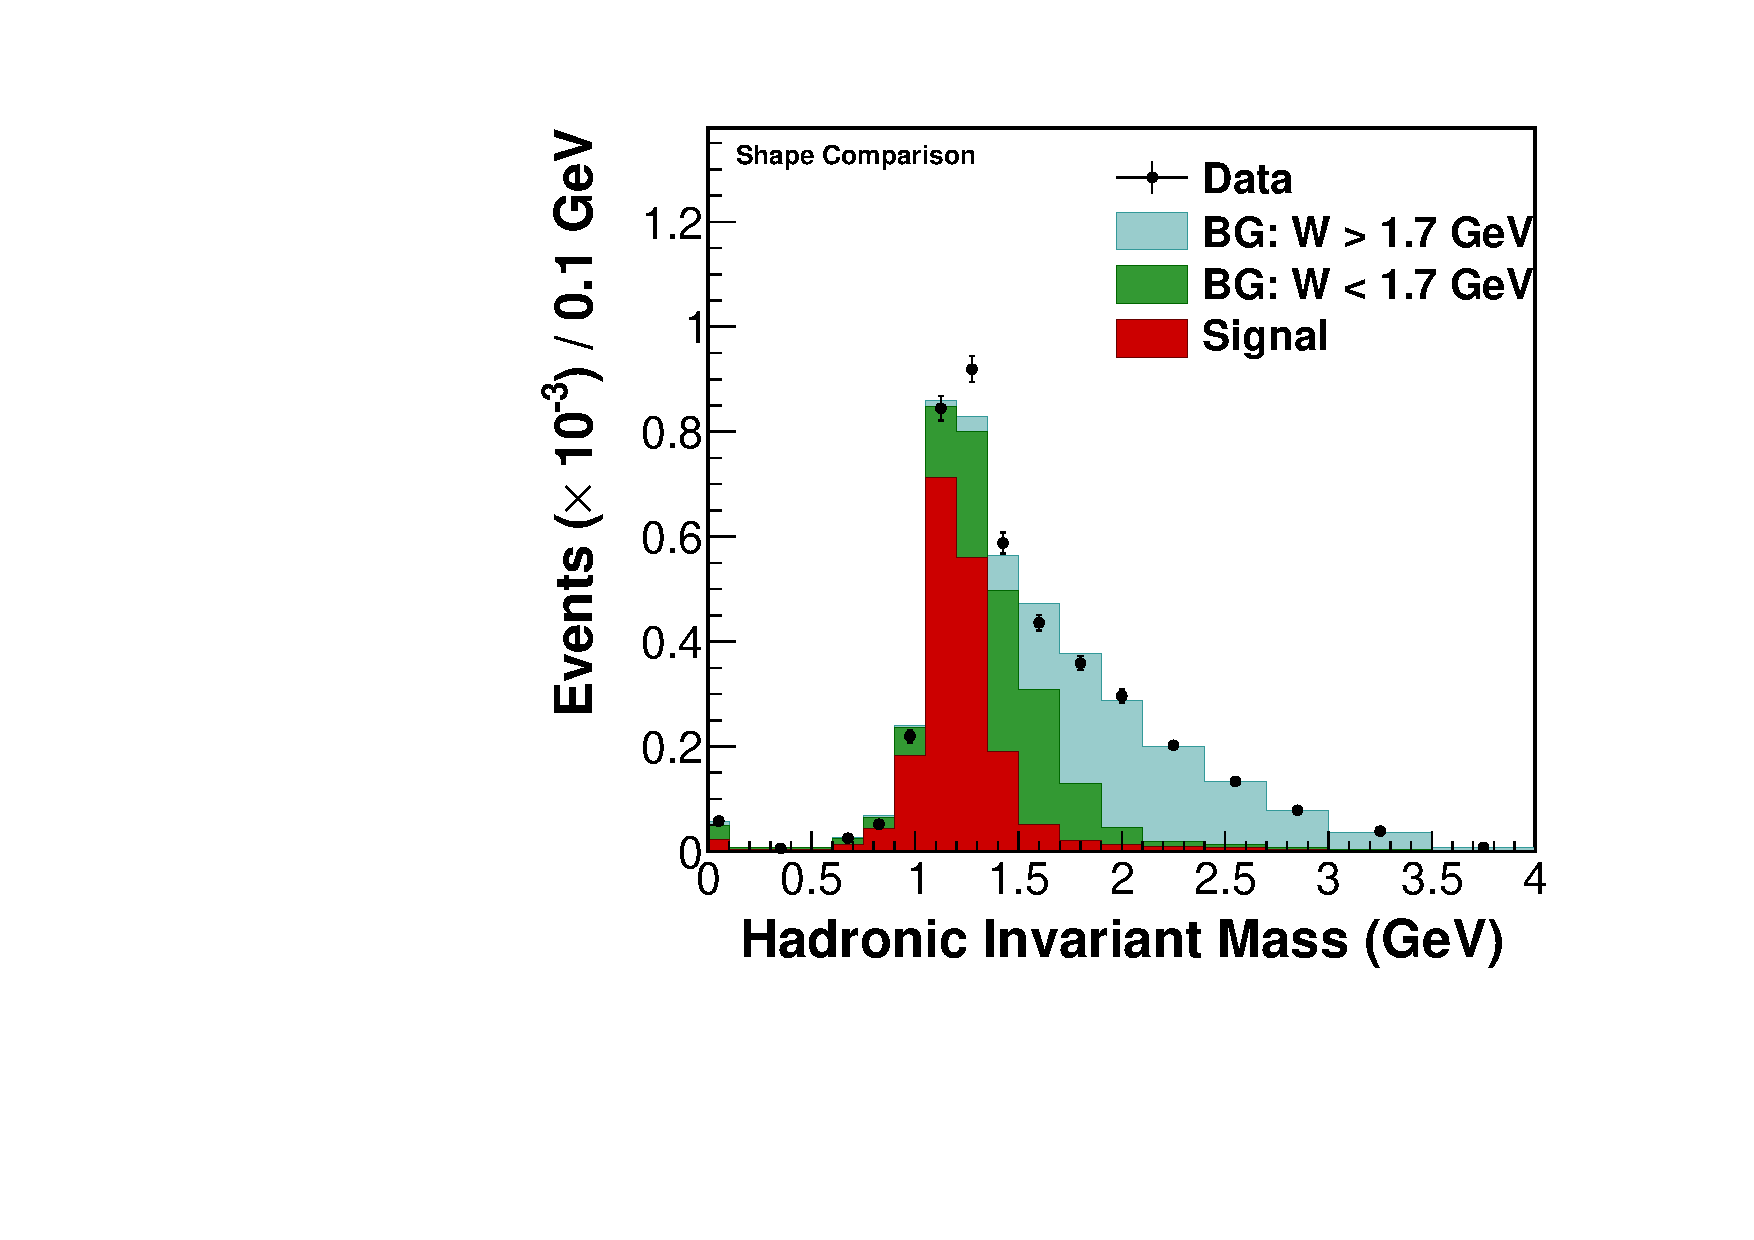
\includegraphics[width=\columnwidth]{figures/WFit_TOTAL_after_pi_ke_1pi}
}
\subfloat[] {
  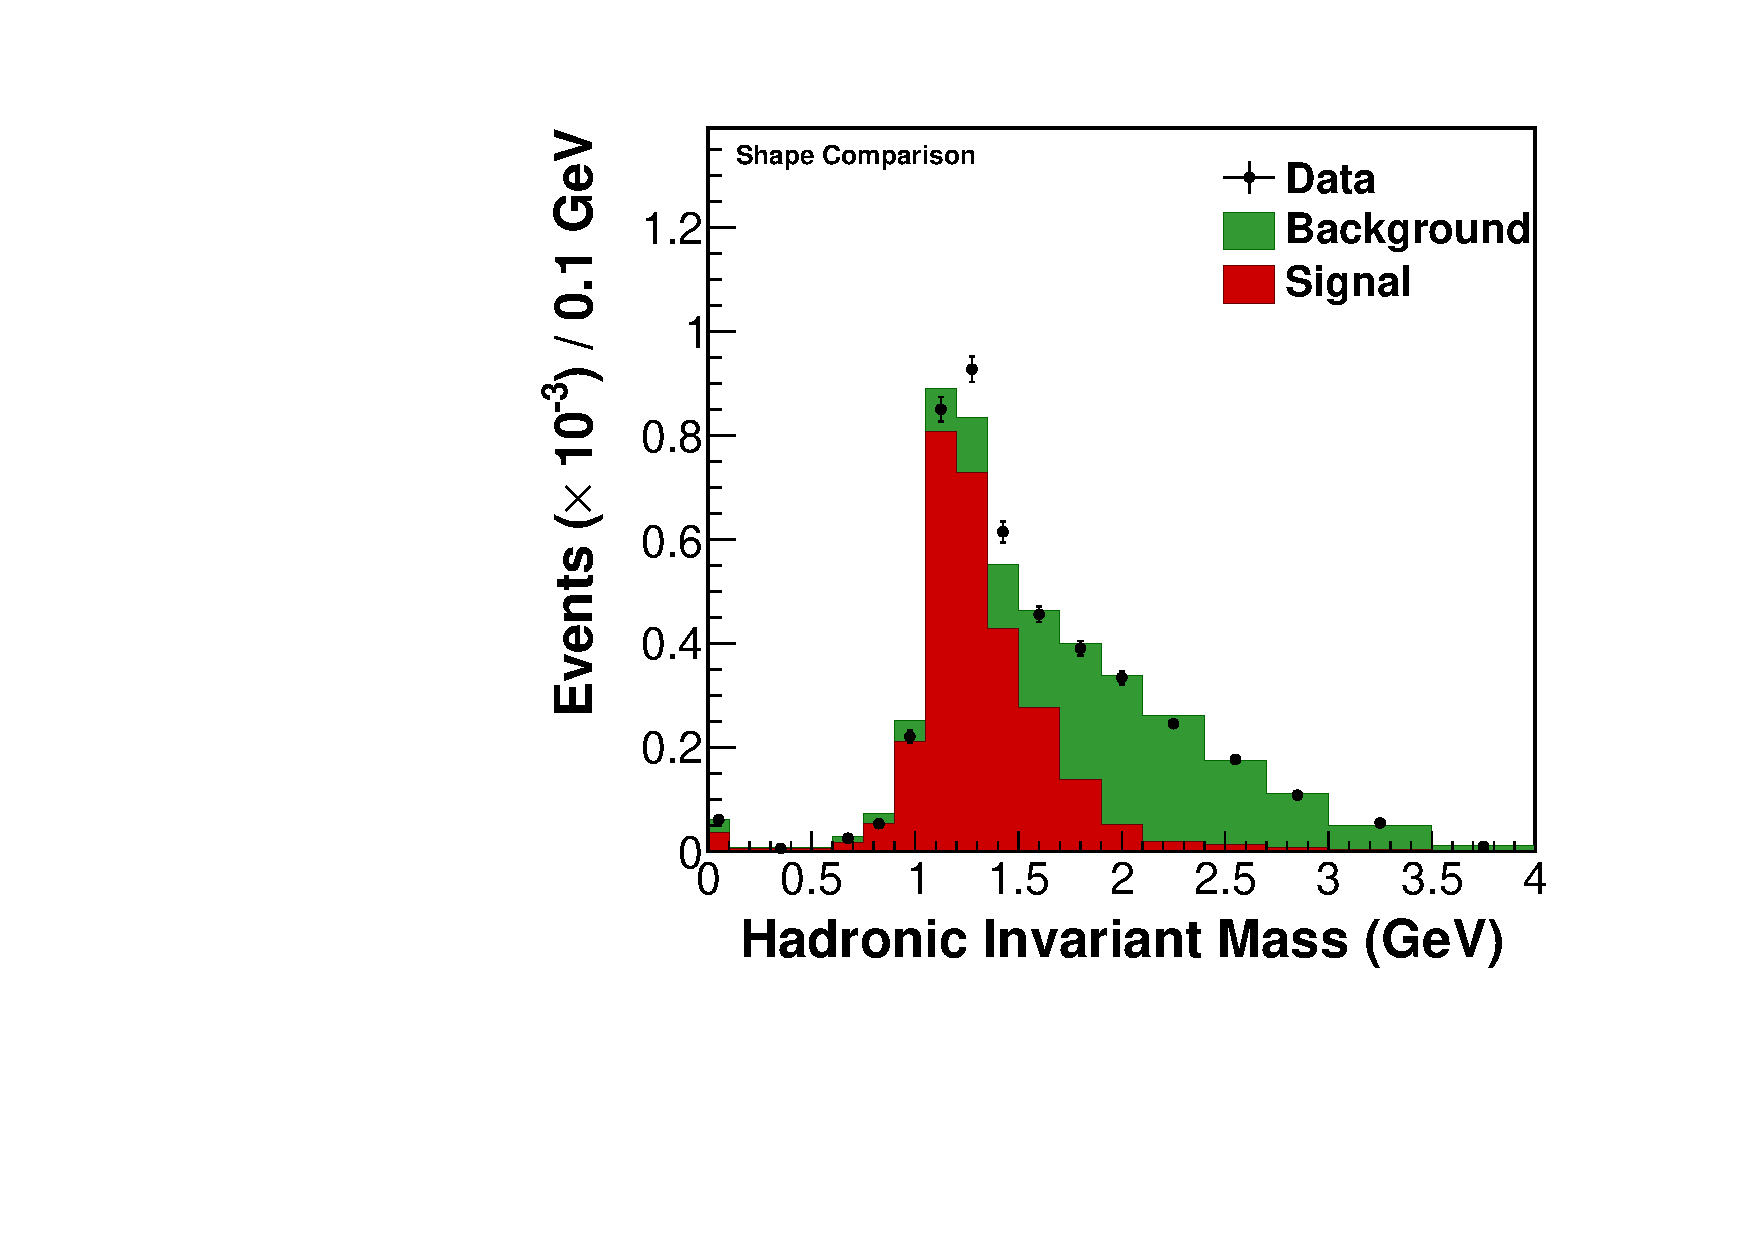
\includegraphics[width=\columnwidth]{figures/WFit_TOTAL_after_pi_ke_Npi}
}
    %\vspace{-7pt}
\caption{The \cconepi (left) and \ccpi (right) $W_{exp}$ distribution after fitting and reweighting the background (BG) and signal templates.  
The events below 100~MeV have a large amount of undetected hadronic energy and are not included in this analysis.}
    %\vspace{-10pt}
\label{fig:Wfit}
\end{figure*}

\subsection{Unfolding}
The background-subtracted reconstructed \Tpi and \thetapi distributions are unfolded using a Bayesian 
procedure~\cite{D'Agostini:1994zf} with four iterations.  The unfolding migration matrix, which determines the probability that 
the true value of a quantity corresponds to a reconstructed value, is derived from simulation.  It is insensitive to FSI effects 
because the true values of \Tpi and \thetapi are calculated at the point where the pion exits the nucleus.  Also, 
the unfolding procedure is not sensitive to normalization uncertainties, including the large uncertainty in the resonance 
production cross section normalization.

The unfolding generally migrates events from low to high \Tpi bins, accounting for the tendency of the reconstruction to report a 
momentum that is too small for pions that interact inelastically in the detector.  The effect of unfolding on 
the \thetapi distribution is small except for the bin at 90$^{\circ}$, where the pion tracking efficiency is poor.  
Some of the pions in the neighboring bins are actually $\sim$90$^{\circ}$ pions that scatter close to the event vertex, 
such that the track reconstruction measures the scattered pion direction.  
The unfolding procedure relies on the GEANT4 interaction model to estimate this effect. 

\subsection{Efficiency Correction}
The efficiency and acceptance correction $\epsilon_{i}$ in Equations~\ref{eq:diffxs} and~\ref{eq:diffxs_ccpi} is calculated according to the
equation

\begin{equation}\label{eq:effdefinition}
\epsilon_{i} = \frac{w_{i}N_{\pi,i}^{S}}{N_{\pi,i}^{T}}, 
\end{equation}
where $N_{\pi,i}^{S}$ is the simulated number of signal pions retained by the event selection, $N_{\pi,i}^{T}$ is the total number of signal pions 
according to simulation, 
and $w_{i}$ corrects for discrepancies in the muon acceptance between data and the simulation.  Data is used to estimate 
other efficiencies, such as the acceptance of the Michel electron selection and the hadron reconstruction efficiencies, but these are found 
to match well to simulation and are included as a systematic uncertainty rather than as a correction.  The muon acceptance is 
compared in data and simulation by forming samples of exiting muon tracks in \minerva and MINOS that point toward the other detector, then 
searching for a matching track in the other detector.  The resulting corrections, which are all between 0.91 and 0.99, are measured separately for each 
data run period so that the time dependence of beam-intensity effects are accounted for.

\subsection{Systematic Uncertainties}
The cross section extraction procedure uses the simulation to estimate backgrounds, detector resolution and acceptance, 
selection efficiencies, and neutrino flux.  The systematic uncertainties on these quantities are evaluated by shifting each parameter in the simulation 
within its uncertainty $\sigma$ to produce a new simulated sample, referred to as an alternative simulation.  The cross sections are remeasured 
using each alternative simulation and a 
covariance matrix is formed from the results.  The covariance matrix for a single systematic uncertainty derived from $N$
alternative simulations is calculated as

\begin{equation}\label{eq:covmx}
C_{ij} = \frac{1}{N}\sum_{n}\left(x_{n,i} - u_{i}\right)\left(x_{n,j}-u_{j}\right),
\end{equation} 
where $i$ and $j$ indicate bins of the differential cross section and $x_{n,i}$ is the measurement of the differential cross section in bin $i$ using 
alternative simulation $n$.  The definition of $u_{i}$ changes according to the value of $N$.  If there is only one
alternative simulation, then $u_{i}$ is 
the value of the cross section measured from the nominal simulation.  Otherwise, $u_{i}$ is the mean of the measured 
cross section in all alternative simulations.  The total covariance matrix is the sum of $C_{ij}$ calculated for each systematic uncertainty.

The computational cost required to produce a new simulated sample for each systematic uncertainty is prohibitive.  Instead, this is 
effectively done for many uncertainties by reweighting the simulation or, in the case of detector resolution and energy scale uncertainties,
modifying the measured values 
event-by-event.  The effects of a few parameters, such as the effective nuclear size and quark hadronization time in GENIE, cannot be correctly estimated 
by either of these techniques.  In these cases, a new simulated sample is generated with the modified parameters.

Shape systematic uncertainties are reported for each measurement in order to mitigate certain large normalization uncertainties, such as the neutrino 
flux uncertainty.  The shape uncertainties are calculated by normalizing the cross section measurement in 
each alternative simulation so that the integrated cross sections measured in the alternative simulation and nominal simulation are equal.  The shape covariance 
matrix is calculated using the renormalized alternative simulation measurements.

Table~\ref{tab:syst-pi} lists the systematic 
uncertainties in the \cconepi analysis grouped according to the uncertainty source; the \ccpi analysis uncertainties are similar.  The total systematic 
uncertainty is between 16\% and 22\%, while the shape uncertainty ranges from from 3\% to 11\% per bin.  For comparison, the statistical uncertainties 
are approximately 3\% to 14\%.  The total uncertainties are generally systematics-limited, while the shape uncertainties are statistics-limited; the one 
notable exception to this trend is the kinetic energy measurement in the lowest bin (35--55~MeV), which is always statistics-limited.

\begingroup
\squeezetable
\begin{table}
\begin{tabular}{cccccccc}
\hline\hline
$T_{\pi}$ (MeV) & I & II & III & IV & V & Total \\
\hline
35 - 55 & 15 (9.7) & 9.7 (2.8) & 6.8 (2.9) & 8.5 (0.5) & 5.5 (2.2) & 22 (11) \\ 
55 - 75 & 12 (4.4) & 9.7 (3.3) & 8.5 (4.4) & 8.6 (0.4) & 4.8 (1.4) & 20 (7.2) \\ 
75 - 100 & 9.9 (4.6) & 8.9 (2.3) & 6.4 (2.8) & 9.0 (0.4) & 3.8 (0.6) & 18 (5.9) \\ 
100 - 125 & 10 (3.4) & 6.8 (1.7) & 4.9 (1.4) & 9.2 (0.7) & 3.0 (0.7) & 17 (4.2) \\ 
125 - 150 & 11 (3.0) & 6.7 (1.6) & 5.0 (1.5) & 8.9 (0.2) & 3.1 (0.4) & 17 (3.7) \\ 
150 - 200 & 11 (3.3) & 6.9 (2.2) & 3.1 (2.8) & 9.1 (0.4) & 2.7 (1.6) & 16 (5.1) \\ 
200 - 350 & 16 (7.2) & 8.5 (1.5) & 4.3 (3.1) & 9.2 (0.3) & 2.9 (1.2) & 21 (8.0) \\ 
\hline
\hline
$\theta_{\pi\nu}$ (degree) & I & II & III & IV & V & Total \\
\hline
0 - 15 & 11 (2.2) & 7.5 (6.7) & 11 (5.8) & 8.8 (0.6) & 4.9 (1.4) & 20 (9.3) \\ 
15 - 22 & 9.9 (2.3) & 9.2 (1.7) & 7.1 (2.3) & 9.2 (0.7) & 3.5 (0.4) & 18 (3.8) \\ 
22 - 29 & 10 (2.0) & 11 (1.8) & 4.4 (2.3) & 9.3 (0.5) & 3.3 (1.5) & 18 (3.9) \\ 
29 - 36 & 10 (1.9) & 12 (2.8) & 4.9 (2.2) & 9.1 (0.4) & 3.2 (1.6) & 19 (4.4) \\ 
36 - 43 & 11 (1.8) & 12 (3.1) & 5.6 (1.6) & 9.0 (0.2) & 3.3 (0.7) & 20 (4.0) \\ 
43 - 50 & 12 (2.0) & 12 (3.0) & 4.7 (1.5) & 9.4 (0.6) & 3.1 (0.8) & 20 (4.0) \\ 
50 - 57 & 12 (2.8) & 12 (3.1) & 3.9 (2.3) & 8.7 (0.6) & 4.7 (1.6) & 20 (5.1) \\ 
57 - 72 & 11 (1.5) & 10 (1.7) & 2.8 (4.3) & 8.6 (0.6) & 3.8 (0.6) & 18 (4.9) \\ 
72 - 108 & 11 (0.7) & 7.8 (1.8) & 6.1 (1.4) & 8.9 (0.2) & 4.4 (0.9) & 18 (2.5) \\ 
108 - 130 & 11 (2.3) & 6.4 (2.9) & 8.3 (4.1) & 9.2 (0.3) & 4.4 (0.6) & 19 (5.6) \\ 
130 - 140 & 9.7 (2.4) & 6.8 (2.6) & 7.7 (4.1) & 9.1 (0.2) & 4.3 (1.2) & 17 (5.5) \\ 
140 - 150 & 9.2 (2.9) & 7.3 (2.2) & 7.4 (3.9) & 9.0 (0.4) & 4.3 (0.6) & 17 (5.4) \\ 
150 - 165 & 9.7 (3.0) & 6.1 (3.2) & 5.6 (3.9) & 9.2 (0.5) & 5.4 (1.9) & 17 (6.2) \\ 
\hline\hline
\end{tabular}
\caption{Fractional systematic uncertainties (in per cent) on \cconepi $d\sigma/dT_{\pi}$ (top) and $d\sigma/d\theta_{\pi\nu}$ (bottom) 
associated with detector response (I), neutrino cross section model (II), nuclear effects including FSI (III), flux (IV), 
and other sources (V).  The absolute uncertainties are followed by shape uncertainties in parentheses.}
\label{tab:syst-pi}
\end{table}
\endgroup


The largest contribution to the total uncertainty comes from uncertainty in the detector response, particularly the average calorimetric response to 
events passing the analysis selections (6-11\%), to which the background-constraining fits are particularly sensitive.  The measurements at low pion 
kinetic energy are also very sensitive to the detector mass model uncertainty (7\% between 35 and 55 MeV) since this affects the pion track 
reconstruction threshold.  The total uncertainty also has large contributions from the neutrino-nucleon cross section model (6-12\%) and neutrino flux 
uncertainty ($\sim$9\%).  The primary uncertainty from the neutrino-nucleon cross section model comes from modeling the muon angular 
distribution in resonance production (7-12\%), which affects the estimated MINOS muon acceptance.  This uncertainty can be reduced to 4\% or less by
restricting the signal definition to muon angles less than $20^\circ$; the Appendix contains the results of this measurement variation.

The shape uncertainties are generally less sensitive to the systematic effects described above, especially to the neutrino flux (reduced to $<$1\%).  The exception to this 
is the measurement at \Tpi between 35 and 55 MeV, which retains sensitivity to the detector mass model.  Additionally, the shapes of the angular 
cross section measurements at forward angles are sensitive to the large uncertainties assumed in the $\Delta$ decay anisotropy model 
(see Section~\ref{sec:expt_sim}).

  





